\documentclass[11pt,a4paper]{report}
\usepackage{graphicx}
\usepackage{color,listings}
\usepackage{dissertation}
\usepackage{enumerate}
\usepackage{float}
% Aberstwyth dissertation LaTeX Template
% Authors: Dr. Hannah Dee (hmd1@aber.ac.uk), Neil Taylor (nst@aber.ac.uk)
% This has been adapted from the Leeds Thesis template and the
% Group Project template for Computer Science in Aberystywth University.
%
% All comments and suggestions welcome.
%
% Template designed to be used with pdflatex: it may need alteration to
% run with a different LaTeX engine

% To build document on the unix command line, run four commands:

% pdflatex dissertation
% bibtex dissertation
% pdflatex dissertation
% pdflatex dissertation

% you will end up with dissertation.pdf
\usepackage{mmp}

% the following packages are used for citations - You only need to include one.
%
% Use the cite package if you are using the numeric style (e.g. IEEEannot).
% Use the natbib package if you are using the author-date style (e.g. authordate2annot).
% Only use one of these and comment out the other one.
%\usepackage{cite}
\usepackage{natbib}

% Use the following to selectively exclude chapters
%\includeonly{cover,abstract,acknowledge,declare,chapter1,chapter2}

\begin{document}

% all of the include directives below refer to tex files
% so 
\title{Arduino based obstacle avoidance robot}

% Your name
\author{Daniel Atkinson}

% Your email
\authoremail{daa9@aber.ac.uk}

\degreeschemecode{G401} %e.g. G400
\degreeschemetitle{Computer Science} % e.g. Computer Science
\degreetype{BSc}

\modulecode{CS39440} % i.e. CS39440, CC39440, CS39620
\moduletitle{Major Project} % i.e. Major Project or Minor Project

\date{1st March 2012} % i.e. the date of this version of the report

\status{Draft} % Use draft until you create the release version. Then, change this to Release.
\version{0.5}

%The title and name of your supervisor.
\supervisor{Dr./Prof. Dave Barnes}

%The email for your supervisor.
\supervisoremail{FIXME@aber.ac.uk}

\maketitle



 includes cover.tex - to change the content,
% edit the tex file

\pagenumbering{roman}

% This is the front page

\title{Arduino based obstacle avoidance robot}

% Your name
\author{Daniel Atkinson}

% Your email
\authoremail{daa9@aber.ac.uk}

\degreeschemecode{G401} %e.g. G400
\degreeschemetitle{Computer Science} % e.g. Computer Science
\degreetype{BSc}

\modulecode{CS39440} % i.e. CS39440, CC39440, CS39620
\moduletitle{Major Project} % i.e. Major Project or Minor Project

\date{1st March 2012} % i.e. the date of this version of the report

\status{Draft} % Use draft until you create the release version. Then, change this to Release.
\version{0.5}

%The title and name of your supervisor.
\supervisor{Dr./Prof. Dave Barnes}

%The email for your supervisor.
\supervisoremail{FIXME@aber.ac.uk}

\maketitle





% Set up page numbering
\pagestyle{empty}

% declarations of originality
\thispagestyle{empty}

%%%
%%% You must sign the declaration of originality. 
%%%
\begin{center}
    {\LARGE\bf Declaration of originality}
\end{center}

In signing below, I confirm that:

\begin{itemize}
\item{This submission is my own work, except where clearly
indicated.  }

\item{I understand that there are severe penalties for plagiarism 
and other unfair practice, which can lead to loss of marks
or even the withholding of a degree. }
 
\item{I have read the sections on unfair practice in the Students' 
Examinations Handbook and the relevant sections of the 
current Student Handbook of the Department of Computer 
Science.}
 
\item{I understand and agree to abide by the University's
regulations governing these issues.}
\end{itemize}

\vspace{3em}
Signature ............................................................  \\

\vspace{1em}
Date ............................................................ \\

%%% 
%%% We would like to make a selection of final reports available to students that take 
%%% this module in future years. To enable us to do this, we require your consent. You 
%%% are not required that you do this, but if you do give your consent, then we will have 
%%% the option to select yours as one of a number of reports as examples for other 
%%% students. If you would like to give your consent, then please include the following 
%%% text and sign below. If you do not wish to give your consent, please remove this 
%%% from your report. 
%%%
\vspace{5em}
\begin{center}
    {\LARGE\bf Consent to share this work}
\end{center}

In signing below, I hereby agree to this dissertation being made available to other
students and academic staff of the Aberystwyth Computer Science Department.  

\vspace{3em}
Signature ............................................................  \\

\vspace{1em}
Date ............................................................ \\



\thispagestyle{empty}

\begin{center}
    {\LARGE\bf Acknowledgements}
\end{center}

I am grateful to...

I'd like to thank...
 % Acknowledgements
\thispagestyle{empty}

\begin{center}
    {\LARGE\bf Abstract}
\end{center}
The aim of this project is to physicaly build and write the software for a robot.  This robot should be able to drive around within its environment under its own power without colliding with any obstruction.  It should also be able to see areas of the environment using some form of sensor system in order to determin which direction to travel safely.
                 % Abstract

\pagenumbering{roman}
\pagestyle{fancy}
\fancyhead{}
\fancyfoot[C]{\thepage}
\renewcommand{\headrulewidth}{0 pt}
\renewcommand{\chaptermark}[1]{\markboth{#1}{}}

\tableofcontents
\newpage
\listoffigures
\newpage
\listoftables
\newpage

% Set up page numbering
\pagenumbering{arabic}

\setchapterheaderfooter

% include the chapters
\chapter{Background \& Objectives}

I was first exposed to electronics in an academic environment in high school.  This was only very basic circuitry, such as making a light flash by using simple integrated circuits.  Being introduced to integrated circuits made building an electronic timer much easier, which was the first thing I produced using these small chips.  This was very satisfying when it finally worked, a feeling I still get when something I make that works as intended.
\\Fast forward to college five years later and I am still fascinated by electronics.  Still using these wondrous little chips to build more interesting circuits I built an audio amplifier whereby I input a waveform into the circuit, either generated by a signal generator or my guitar, and amplify it or smooth the signal to create a new sound, then output this amplified signal to a speaker.  This distorted sound is similar to those created by a guitar amplifier that has built in effects or an specific effects pedal also used by guitarists.
\\At college I also took a computing class in which the programming language Visual Basic was taught as part of the course.  Naturally the next step would be to combine the electronics with the programming knowledge.  This took the form of a small blinking light project where I use a PIC (Peripheral Interface Controller) to flash an LED (Light Emitting Diode).  A PIC is a small chip (Integrated Circuit) which can run small amounts of code to read inputs and control outputs on its various pins.
\\In the summer between the end of College and starting University I discovered a range of open source hardware microcontrollers called Arduino.  These boards made combining program code and electronic hardware much easier by doing much of the base work for me.  These microcontrollers have a large community, which has written all forms of libraries to interface the board with various pieces of hardware and control them with much less effort than would be needed when using a PIC.  The PIC does have a large variety of libraries but the Arduino seems to have a much wider variety of what is supported and a very active community to help if you get stuck.
\\I have also had some experience using the pioneer research robot created by Adept MobileRobots \cite{mobilerobots} which are used by Aberystwyth University in the robotics lab.  The experience with these robots was to use their ultrasonic sensors to try and avoid hitting some polystyrene boards.  Due to the limited time available to use these robots the resulting code was not very effective or polished, but it has heavily influenced my ideas for designing my current project and further pricked my enthusiasm for robotics and all of the possible applications it has.
\\\\My main objective with this project is to produce a piece of hardware that can manoeuvre itself around an environment under it's own power without bumping into anything.  This is to be built utilising the knowledge I have gained about electronics and programming from previous projects and from the courses I have attended as part of my University degree.


%\addcontentsline{toc}{chapter}{Development Process}
\chapter{Development Process}

You need to describe briefly the life cycle model that you used. Do not force your project into the waterfall model if it is better described by prototyping or some other evolutionary model. You do not need to write about all of the different process models that you are aware of. Focus on the process model that you have used. It is possible that you needed to adapt an existing process model to suit your project; clearly identify what you used and how you adapted it for your needs.

In most cases, the agreed objectives or requirements will be the result of a compromise between what would ideally have been produced and what was felt to be possible in the time available. A discussion of the process of arriving at the final list is usually appropriate.

You should briefly describe the design method you used and any support tools that you used. You should discuss your choice of implementation tools - programming language, compilers, database management system, program development environment, etc.

\section{Introduction}
I chose to use the iterative and incremental approach to development.  This is mainly because of how modular my project is.  In theory, I can add more functionality with minor adjustments to the core system, thus making iterative/incremental very suited to my needs.
\\Each part of the system in an incremental strategy can be developed independently and slotted together as they reach completion.
\\Each iteration is a review of the previous which has been reworked and improved upon.
\\For a well functioning system it needs good design, quality programming and a good debugging process.  So, after designing the inital system, writing a simple prototype it is then time for debugging it to get an indication of what the main flaws are.  Once these flaws have been clearly identified a new design has to be drawn up to correct these issues.  After writing the new version following the revised design the cycle continues in the same manner, design, write then debug.


\section{Modifications}
No real modifications were made to this development process as it works for individuals and for teams without alteration.

\section{Version Control}
This is majorly usefull in any project that involves managing code or documents digitaly.  It is even usefull as a backup tool, to be safe from accidental deletions, hard drive failure or any number of unfortunate occurances as you can just re-download the files.
\\The other features that version control systems offer as of more use in this type of project.  Branching and merging are two of the most used features.  These enable the user to make a branch within the project in which they can work on a specific feature independantly of the main project.  You may make multiple branches at the same time and work on different things all independant of each other.  Once these are finished you can merge them back into the main project, this is a very nice feature version control systems offer as it performs most, if not all of this for you, instead of having to manualy try and integrate each line of the branch files back into the main ones.
\\I have chosen to use Git for developing this project due to how powerful the merge feature is as well as a website called github \cite{github} which will host repositories for people.  The website also has nice usage statistics and offer some private repositories to students.  Github repositories are normally open to the general public unless you pay a fee for having non public facing ones, being a student enables me to have a small number of these private ones which let em control when I am ready to release a project to public viewing.


\chapter{Design}



%You should concentrate on the more important aspects of the design. It is essential that an overview is presented before going into detail. As well as describing the design adopted it must also explain what other designs were considered and why they were rejected.

%The design should describe what you expected to do, and might also explain areas that you had to revise after some investigation.

%Typically, for an object-oriented design, the discussion will focus on the choice of objects and classes and the allocation of methods to classes. The use made of reusable components should be described and their source referenced. Particularly important decisions concerning data structures usually affect the architecture of a system and so should be described here.

%How much material you include on detailed design and implementation will depend very much on the nature of the project. It should not be padded out. Think about the significant aspects of your system. For example, describe the design of the user interface if it is a critical aspect of your system, or provide detail about methods and data structures that are not trivial. Do not spend time on long lists of trivial items and repetitive descriptions. If in doubt about what is appropriate, speak to your supervisor.


\section{Overall Architecture}
The initial design for the robot is to produce a small vehicle capable of moving freely within an environment under it's own power with a platform for mounting the various systems.  These systems should be a central control unit, motor control and the various sensors.

\begin{figure}[H]
\centering
        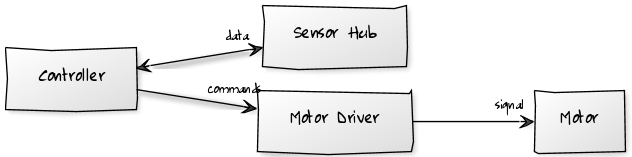
\includegraphics[width=4.0in] {Images/basic-uml.png}
        \caption{Basic system diagram}
        \label{Basic system diagram}
\end{figure}


\begin{figure}[H]
\centering
        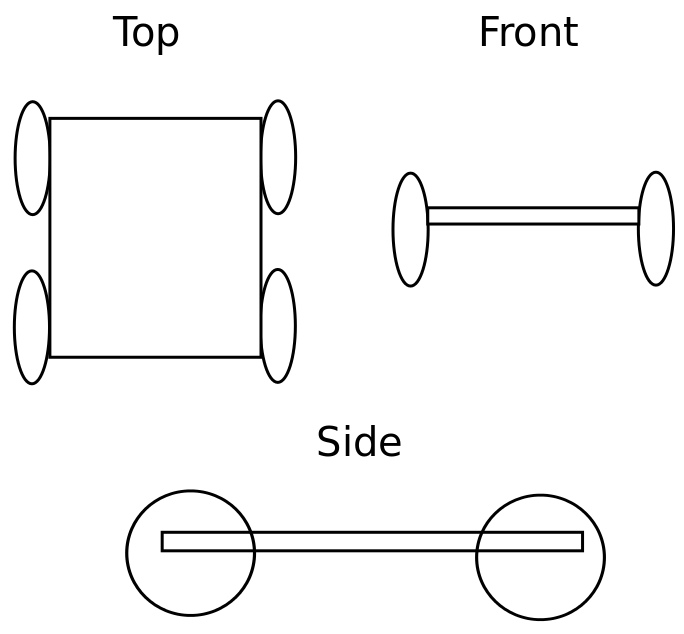
\includegraphics[width=2.0in] {Images/initial-design.png}
        \caption{Initial design}
        \label{Initial design}
\end{figure}

The central control unit will be a microcontroller for ease of interfacing directly with hardware as well as keeping power consumption down.  Keeping power consumption to a minimum is important so that the robot can be active for a longer period of time without needing to be recharged.  This controller will interface with both a motor control system and the various sensors required to detect objects in the environment local to the robot.

\section{Design Research}
The various components that the project will need to come together into a finished product have many different possible options to choose from, all with their various strengths and weaknesses.
\subsection{Materials}
There were several considered materials for the robot chassis to be built of and the ideal material would be:
\begin{enumerate}
\item Extremely difficult to break so that it does not get damaged easily while in use.
\item As light as possible to make it easier on whichever drive system is used to move it.
\item To be as low cost as possible so that it is affordable to a student.
\item Something that does not conduct electricity which could possibly damage an electrical component mounted onto it.
\item Hard to bend to avoid being bent out of shape by any possible heavy load the robot may end up carrying or colliding with.
\item Easy to cut so that it is possible to craft into the required shape.
\end{enumerate}

\begin{itemize}
\item Wood
\\This would be the easiest material to make the chassis from as it is very cheap, easy to cut into the intended shape and easy to mount components on with either adhesive, nails or screws.  Also the fact that it does not conduct electricity will help when mounting circuit boards to it.

\item Plastic
\\The lightest option.  Good due to its low weight but may not be as strong as wood or a metal option and could bend or snap under the load of heavier components such as motors or a large power source.  It can be more expensive than wood to acquire.  There is a higher difficulty in cutting it into the desired shapes.  It is also non-conductive, again useful to mount electronic components to.  Plastic can hold a static charge which can be damaging to electrical components.

\item Steel
\\A stronger material that can withstand a much heavier load than wood of plastic. It may be able to withstand a heavier load before it is bent out of shape but is itself more heavy than the weaker options of wood or plastic.  This extra base weight before adding anything else will put more strain onto which ever drive system that is used to drive the robot and may even need to use more powerful motors because of this extra weight.  It is a very conductive material which means that a non-conductive mounting platform will also be needed to mount electronic components as to avoid damaging them.

\item Aluminium
\\A much lighter metal than steel, but still much heavier than wood or plastic or the same thickness.  It can also withstand heavier loads than wood or plastic but it also much more difficult to cut.  Again aluminium is a very conductive material meaning that a non-conductive mounting platform will be needed.  It can also be used as a heat sink for the components that can get very hot such as the motor drivers or the motors themselves.  A heatsink is a material attached to something that gets very hot and conducts that heat.  It generally has a large surface area to dissipate the heat into the cooler air around it, but it may also have a fan to blow/draw the hotter air away replacing it with air/gas with a lower temperature than that of the heatsink.

\end{itemize}

Aluminium seems to be the best all round choice being strong but not as heavy as steel.  It can act as a heat sink if the motors are mounted directly to it.  It is also not very expensive to buy in small amounts.
\\In addition to the aluminium base I have decided to use plastic for mounting components to the base as it is light, inexpensive and non conductive which is suitable for electronic components.

\subsection{Actuators}
Actuators are motors used for controlling movement of a system.  The ideal actuator would be something that:
\begin{enumerate}
\item Has little to no power consumption which will increase the overall total runtime of the robot by decreasing the energy draw on the system.
\item Has as much torque as possible to make moving a larger mass less effort.
\item Weighs as little as possible to reduce the overall weight of the robot.
\item Is as low cost as possible again to be affordable to a student building this robot.
\item Has perfect precision in order to know exactly what position it is in at any time.
\item Have no limits on rotation as some actuators can only turn a set amount before having to turn back.
\item High speed range so that it can move as slow as needed or as fast as needed.
\item No wear and tear for easy or no maintenance.
\end{enumerate}
\begin{itemize}
\item Servo
\\Typical servos are a motor and a gearbox with a potentiometer, a voltage divider in this case used to determine how far a motor has turned, for feedback.  These motors are great for controlling such things as the direction of sensors or moving very light devices.  Servos are low voltage, typically 4.8 - 6 volts, and as such do not have much strength, which means that they are typically not good for driving larger equipment.  Additionally most servos only turn up to 180 degrees or 360 degrees.  In normal operation they do not turn continuously but can be modified to do so at the cost of losing the feedback of how far the motor has turned.
\begin{figure}[H]
\centering
        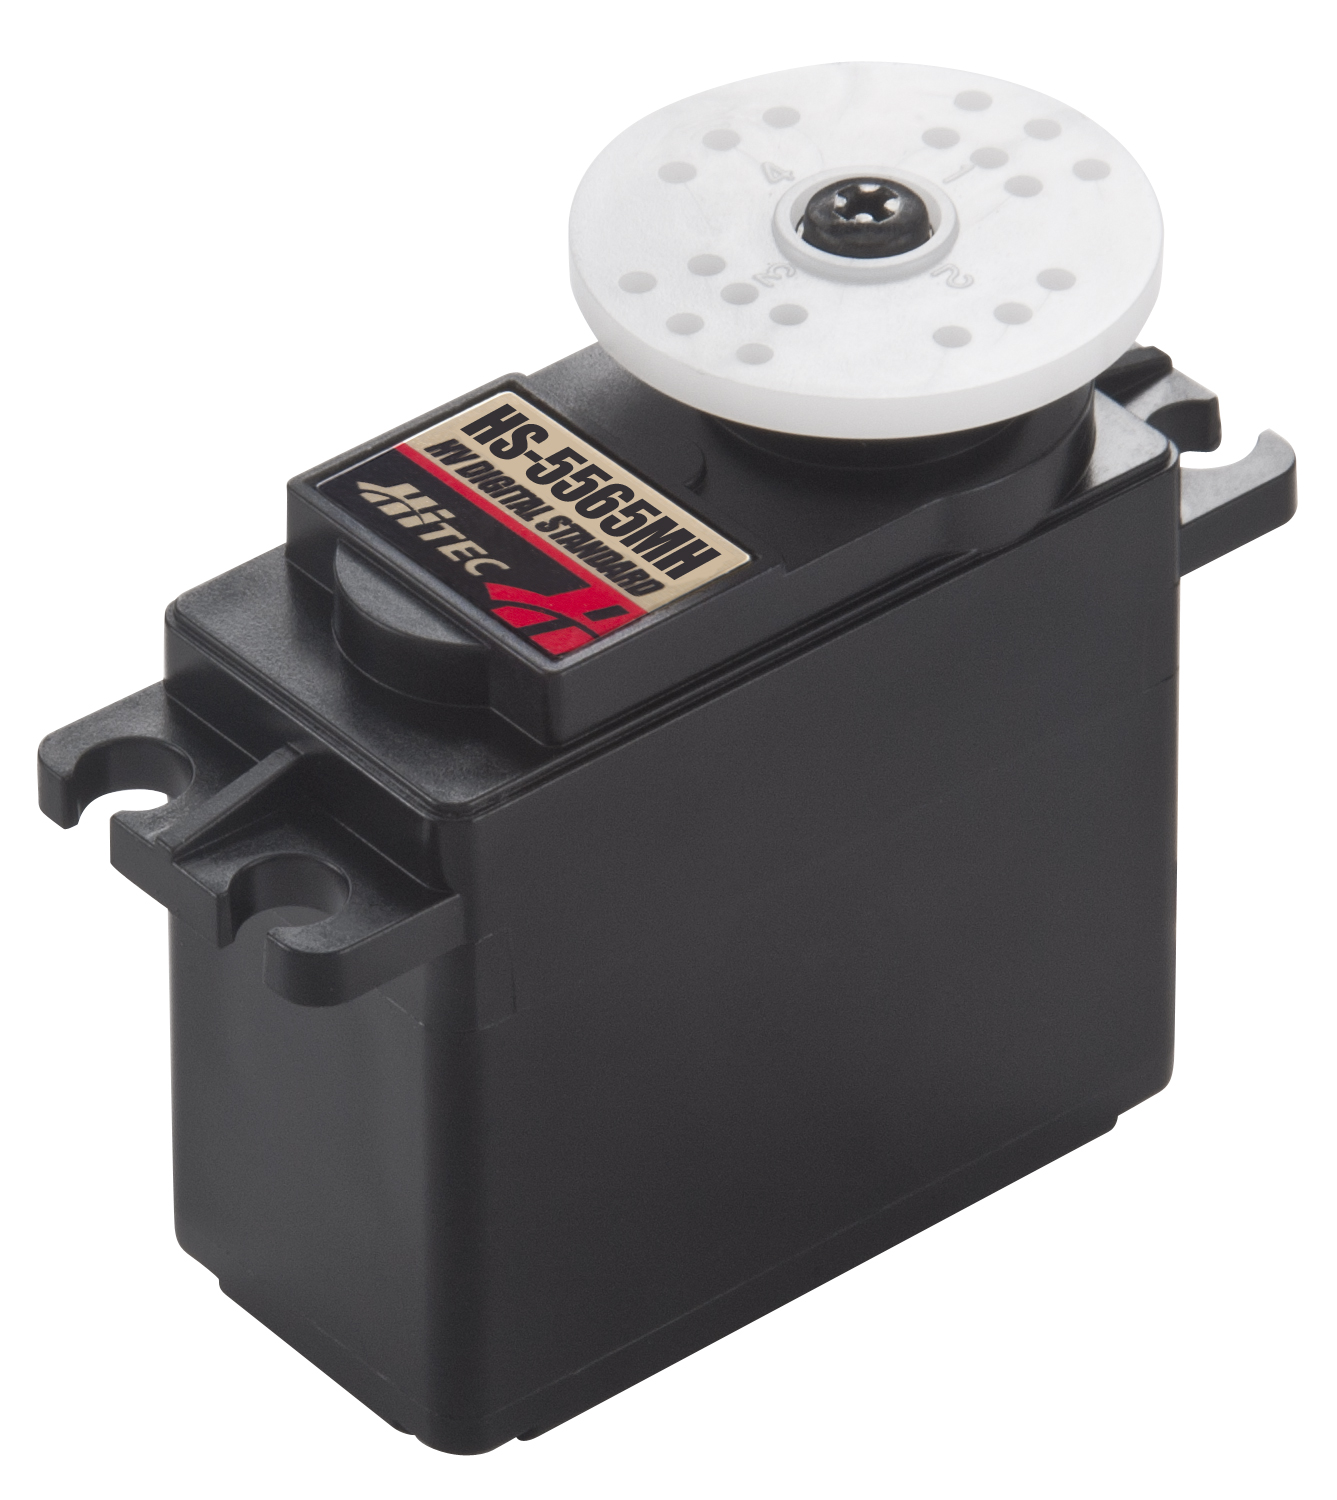
\includegraphics[width=1.5in] {Images/servo.jpg}
        \caption{Servo Motor - robotshop.com}
        \label{Servo Motor}
\end{figure}

\item DC Motor
\\Direct current motor has a very simple operation: apply current to one side of the motor to make it turn, reverse the direction of the current to reverse the direction the motor turns.  Changing the speed of these motors is simple, either change the voltage (keeping it within the devices tolerances) or turn the current supplied to the motor on and off at high speed where how quickly it is alternated determines the speed of the motor.  Typically these motors are attached to a gearbox to gain more torque to drive much higher loads.  Optical rotary encoders can be used to determine how much the motors have turned and how fast.  An optical rotary encoder can be fitted to any motor to add the functionality of positional feedback.  These encoders use a light based sensor to detect when the light changes in front of it, this can be used with a disc that has black and white lines on it.  The change in color is detected, this along with how many times it changes and with what frequency this happens can determine the amount a wheel has turned and how fast it has done so.
\begin{figure}[H]
\centering
        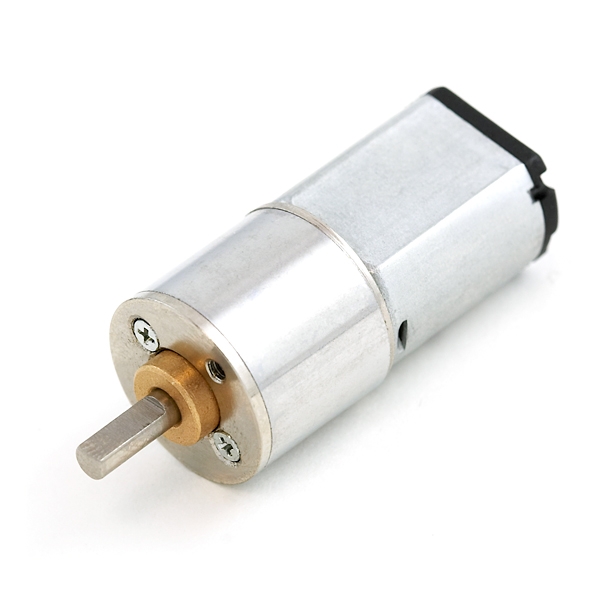
\includegraphics[width=2.0in] {Images/dc-motor.jpg}
        \caption{DC Motor - sparkfun.com - CC BY-NC-SA 3.0}
        \label{DC Motor}
\end{figure}
\item Steppers
\\Stepper motors use an internal gear and a ring of magnets.  These magnets pull the gear into position, powering the magnets in sequence which will turn the motor.  Each part of this cycle is called a step.  This means that a single step is a known amount of rotation.  Using this type of motor ensures that you can accurately turn whatever is attached to the motor shaft by a known amount without any additional measuring equipment.  But adding any such measuring equipment can add verification to determine if the motor has actually rotated by the amount expected.
\begin{figure}[H]
\centering
\begin{subfigure}
	\centering
        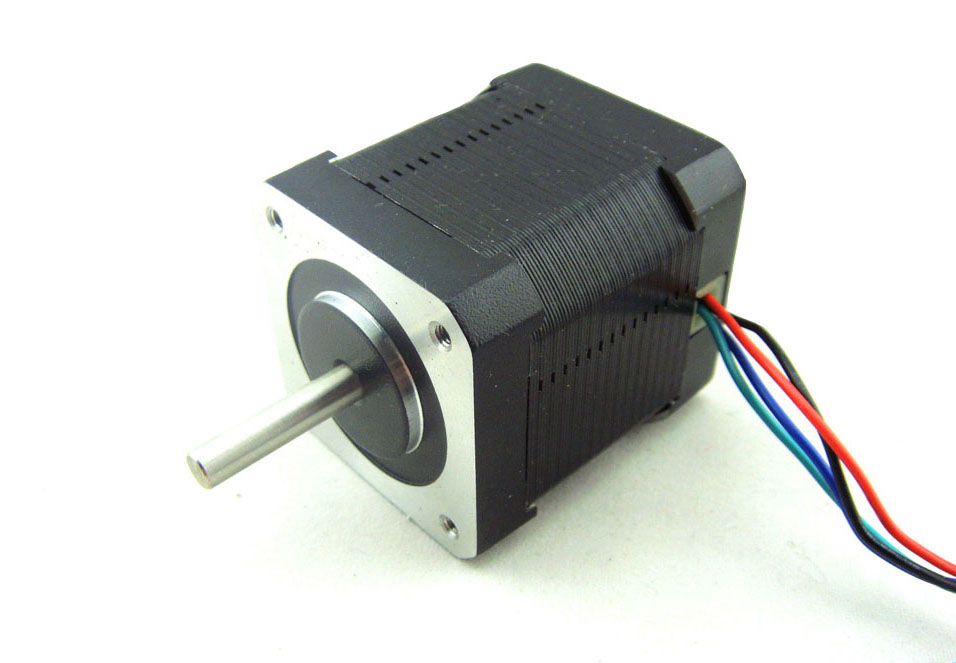
\includegraphics[width=2.0in] {Images/stepper.jpg}
        \caption{Stepper Motor - stepperonline.com}
        \label{Stepper Motor}
\end{subfigure}
\begin{subfigure}
        \centering
        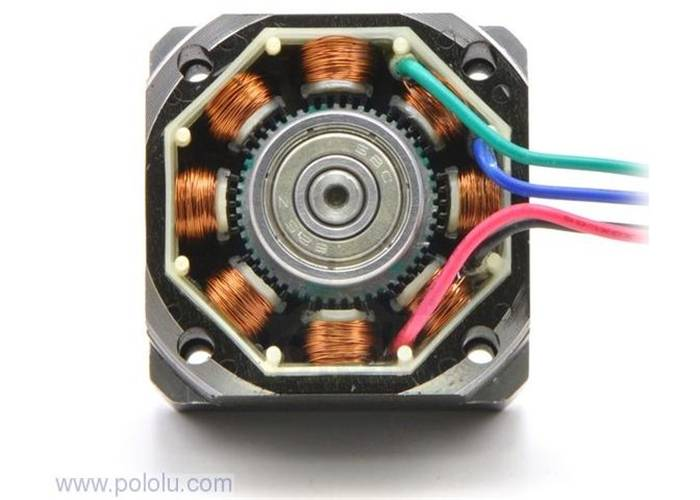
\includegraphics[width=2.0in] {Images/stepper-internal.jpg}
        \caption{Stepper Motor Internal- robotgear.com.au}
        \label{Stepper Motor Internal}
\end{subfigure}
\end{figure}
\end{itemize}

I have chosen to use stepper motors due to the ability to control the amount and speed of rotation with more accuracy than the alternatives.  Stepper motors do come in high torque version which may be needed for this project as the chassis is made of metal which is a much heavier material.  A stepper motor could be used with a chassis of any of the materials mentioned, it may struggle with steel depending on how thick of a piece is used.  DC motors could also be used with all materials if in conjunction with a gearbox, but the additional system needed to measure and control the exact rotation of the wheels using this method puts me off of the idea.  Greater power but less accurate control.
\subsection{Drive Type}
There are various different ways to move a mass around.  The ideal drive system should be:
\begin{enumerate}
\item A very low mass to reduce overall load on the system.
\item Capable of omni-directional movement to increase the ease of moving within confined environments.
\item Perfectly stable so that the robot doe snot fall over or collapse.
\item Have high traction as to not slip on it's environment.
\end{enumerate}
No single drive system is going to be perfect in all aspects.
\begin{itemize}
\item Wheels
\\These are most conventional method of movement which are seen by most people every day.  Robots that use wheels to enable movement are often very stable and can be using in many configurations.
	\begin{itemize}
	\item Two Wheels
	\\This is an unstable configuration which requires it to be in constant motion to maintain an upright position.  When configured with the wheels side by side the center of gravity will be directly in the middle between the wheels underneath the axle where a weight is often positioned to help keep it upright as well as a tilt sensor to help compensate for movement.
\begin{figure}[H]
\centering
        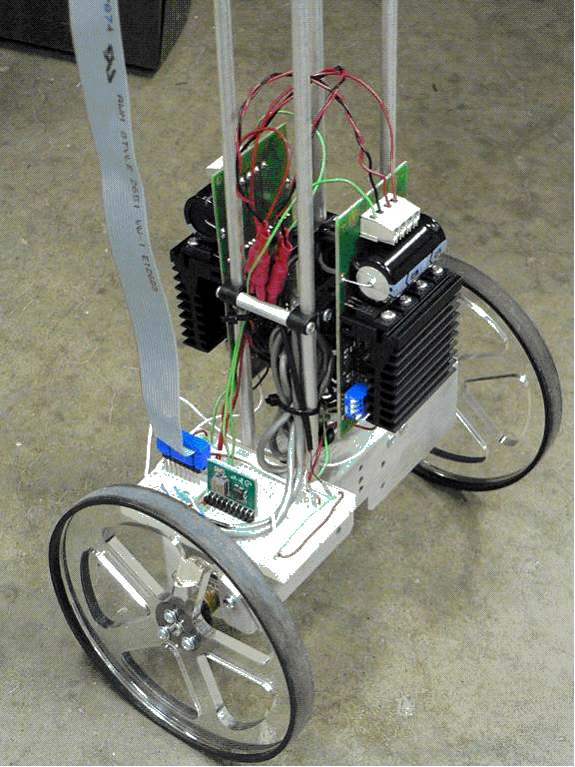
\includegraphics[width=2.0in] {Images/2-wheel-side.png}
        \caption{2 Wheel Gyroscope - ni.com}
        \label{2 Wheel Gyroscope}
\end{figure}
Another way for a two wheels to be arranged would be like a bike where again it will need to be in constant motion to remain upright.


	\item Three Wheels
	\\Most commonly two drive wheels and a single free turning wheel for stability.  To turn the wheels are either turned in the opposite direction of each other or in the same direction just as different speeds using the free turning wheel to stop it falling over or being pulled along the ground as long as the center of gravity if within the three wheels.

	\item Four Wheels
	\\All four wheels can have independent control for tank style movement.  This is harder to keep in a straight line due to having to try and keep all four wheels turning at the same speed otherwise risk being inefficient and also causing additional friction dragging one side back.  An advantage to having all four wheels operated independently is that if using in conjunction with 'omni' wheels.  These wheels have rollers on them enabling then to traverse in a lateral direction if the front and back pair are rotated in the opposite direction of each other.
	\\Car type configuration is also four wheels but only either the front or the back pair are powered and either the front of back pair are able to turn.  Both the wheels that are able to change direction and the powered drive wheels can be the same pair.  It will require some kind of servo system to turn the axis which is designated at the turning wheels.

	\item More than Four Wheels
	\\Very good for uneven terrain as each wheel can rise and fall independently with less effect on the main structure.  These are far more complex to operate but if the terrain is very rocky then it may be the best choice.
	\end{itemize}

\item Tracks
\\These are very stable and have the best traction compared to wheeled variants as long as the surface it is used on is not smooth, sand is a good place to use tracks due to the large surface area compared to wheels as they will not sink while wheels will.  Very high friction with the ground especially when turned as it has to operate the tracks in the opposite direction of each other forcing its way around in a circle.
\begin{figure}[H]
\centering
        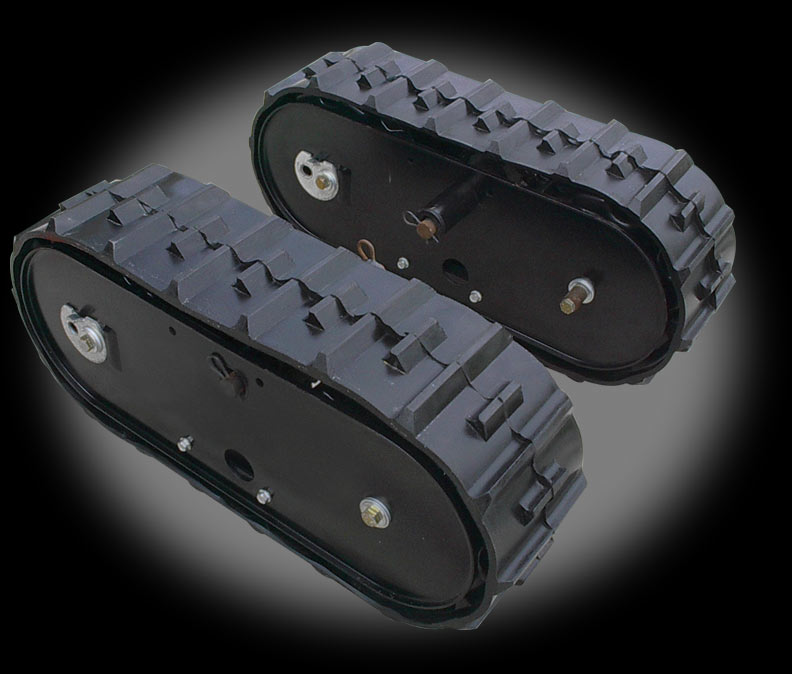
\includegraphics[width=2.0in] {Images/wheel-track.jpg}
        \caption{Tracks - robotcombat.com}
        \label{Tracks}
\end{figure}


\item Legs
\\These are the most uncommon of the movement types.  Due to the cost of developing systems using this type of movement and the overall complexity of controlling them.
	\begin{itemize}
	\item Single Leg
	\\The most difficult to control due to having to balance its load upright on a single point and having to lean in the direction it needs to go without falling over and 'hop' to move around without falling over when landing.
\begin{figure}[H]
\centering
        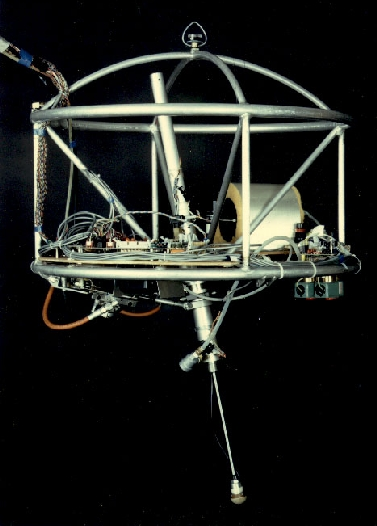
\includegraphics[width=2.0in] {Images/3d-hopper.jpeg}
        \caption{3D One Legged Hopper - mit.edu}
        \label{3D One Legged Hopper}
\end{figure}
	\item Two Legs
	\\Extremely difficult to control and there are very few working practical applications of a two legged robot.  The main issue for controlling this is keeping it upright and not overbalancing, also if knee type joins are added the complexity significantly increases.
	\\Also the mere fact that work on two legged robots is being done by a cutting edge engineering company like Boston Dynamics \cite{boston} is evidence that this kind of system is a fair bit beyond the scope of an undergraduate student project.

\begin{figure}[H]
\centering
        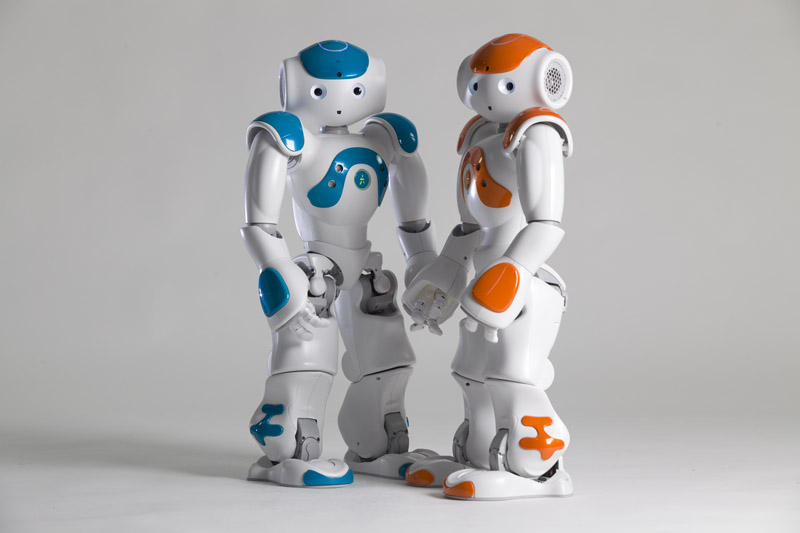
\includegraphics[width=4.0in] {Images/nao.jpg}
        \caption{NAO - aldebaran-robotics.com}
        \label{NAO}
\end{figure}
	\item More than Four Legs
	\\Having more legs can increase stability.  This is because most of the legs can be firmly on the ground while the others are moving into their new position.  Turning can be more complicated to control than the walking already is.  The servos used to control each of these legs and all the joints the legs may have may need to be quite strong or at least have strong teeth as to not get stripped under the weight of whatever payload the robot may have on top of all of these legs.  This is based on how insects are constructed where their body is vastly bigger than its legs, and as such it has many legs to compensate for this and distribute the load.
	\end{itemize}
\end{itemize}
I have decided to use a four wheel configuration to take advantage of the level of traction four wheels will give the robot as well as the added stability over the two or three wheeled configuration.  The configurations with more than four wheels have added complexity in how to control all of the extra wheels and the advantages of having the added wheels are not needed in this project.  Also the legged variety of drive systems are well beyond the scope of this project and the added complexity would not bring any real benefits tot he robot for it's intended purpose of avoiding obstacles in the environment.
\subsection{Sensors}
Sensors are needed so that the robot is able to see what is in the environment around it, enabling it to see, calculate and avoid obstacles.
\\An ideal sensor would be:
\begin{enumerate}
\item Infinite range, being able to see as far as possible and as close as possible.
\item Can no be interfered with, able to be used in any environment and nothing can interfere with the readings it provides.
\item Little to no processing required to acquire and interpret the data provided by the sensor.
\item Lightweight as to not increase load on the drive system.
\item Small so that many can be fitted into a small space for maximum obstacle sensing ability.
\item Cheap as possible to be able to afford many.
\item High resolution as to be able to determine what exactly the objects in the environment are.
\end{enumerate}
Such a wonderful sensor does not exist but there are many options.
\begin{itemize}
\item Bump Skirt
A bump skirt is multiple touch sensors such as buttons arranged like a skirt around the edge of the robot.  When the robot bumps into something the button is pressed telling the robot where it bumped into something.  From this it will be able to move in the appropriate direction to get away from the object it hit.  This is a very bad way of avoiding an obstacle because to know that something is there it will have to hit it first.

\item LDR
\\An LDR is a light dependant resistor.  A small resistor that changes its resistance depending on how much light it is exposed to.  This could be used to detect if the robot is very close to bumping into an object and avoid it as the object got closer and possibly cast a shadow onto the sensor reducing the amount of light the resistor can detect, similar to a physical bump skirt which activates when something touches it.
\begin{figure}[H]
\centering
        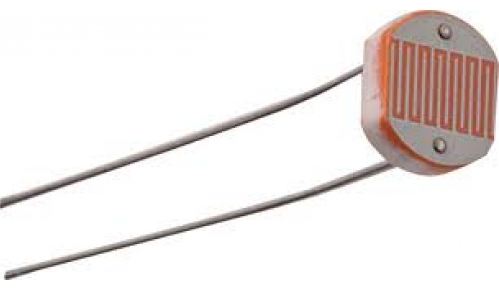
\includegraphics[width=2.0in] {Images/ldr.jpg}
        \caption{Light Dependant Resistor - robotics.org.za}
        \label{Light Dependant Resistor}
\end{figure}

\item Camera
\\A camera could be used to detect objects in front of it by using various image processing techniques to analyse the data it provides.  This method is good because it can potentially map a relatively large area in a single image.  However it requires more processing to do so, which can be slow and result in colliding into an object or being stuck in a tight space before the system has finished processing data from the camera.  This method would force me to use a more powerful processor to overcome the limits of the lower speed processor models but it adds complexity to the project as well as additional cost and a higher power consumption.
\begin{figure}[H]
\centering
        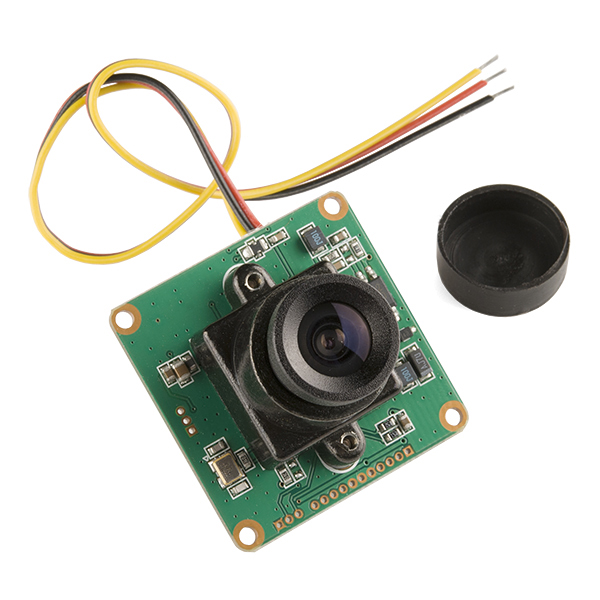
\includegraphics[width=2.0in] {Images/camera.jpg}
        \caption{Camera Module - sparkfun.com - CC BY-NC-SA 3.0}
        \label{Camera Module}
\end{figure}

\item Infrared
\\Used to detect distance from an object.  An emitter and a receiver pair linked to work like the light dependent resistor but using infrared instead of normal visible light.  Depending on the intensity of infrared picked up by the receiver it can be used to determine the distance from the source of the reflection.  Ambient infrared can effect readings as there is infrared radiation emitted from the sun and is everywhere.  This extra radiation other than the amount emitted by the sensor is unneeded and unwanted and as such if it arrives at the receiver it will provide false readings, therefore this can be very inaccurate.
\begin{figure}[H]
\centering
        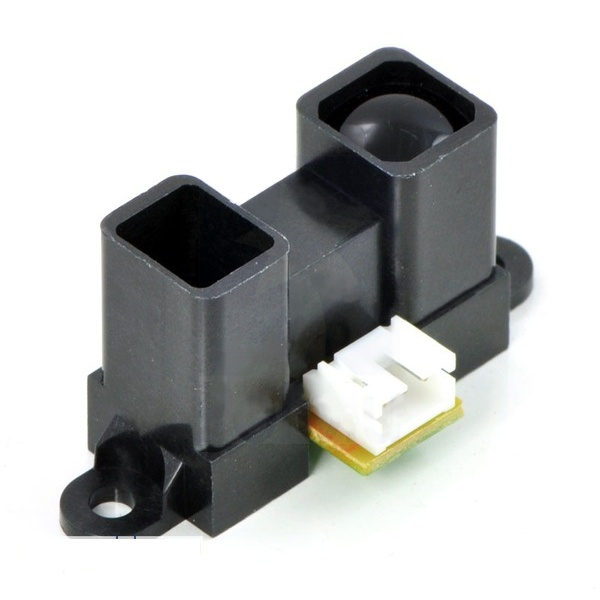
\includegraphics[width=2.0in] {Images/ir.jpg}
        \caption{Infrared Sensor - coolcomponents.co.uk}
        \label{Infrared Sensor}
\end{figure}

\item Sonar
\\An emitter style approach.  It emits an ultrasonic wave to bounce off of whatever surface is in front of it.  The time taken from emitting the wave until receiving the wave determines how far away the object is.  This method comes with its drawbacks.  Due to how sound waves behave when they interact with the environment by bouncing off of it.  If the surface is angled or curved the sound can bounce away from the receiver, either not reaching it at all giving the possible false reading that there is nothing in front of it, or it could bounce off of multiple surfaces back to the receiver giving a false reading that an object is there but further away due to the sound taking longer than it should have to reach the receiver.
\begin{figure}[H]
\centering
        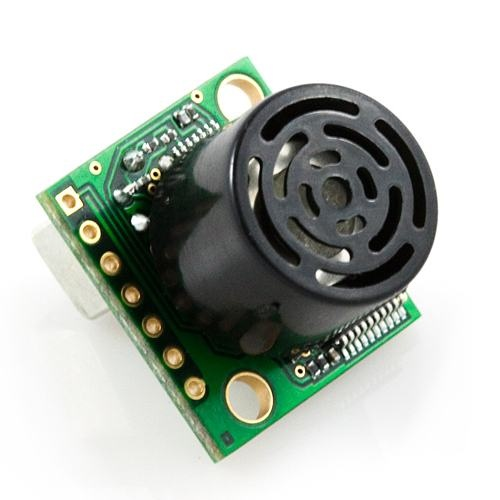
\includegraphics[width=2.0in] {Images/sonar.jpg}
        \caption{Ultrasonic Sensor - coolcomponents.co.uk}
        \label{Ultrasonic Sensor}
\end{figure}

\end{itemize}
A combination of both sonar and infrared logically seems like a good idea.  One can compensate for the others weaknesses.  Use the sonar to compensate for ambient infrared and the infrared can be used to compensate for sonar bouncing around the environment.  Hopefully this will reduce the number of false readings produced.  This does not remove the significant weaknesses of ambient infrared or the sonar echo but should help identify which readings are being affected by comparing the two different readings taken by the different sensor types.
\subsection{Control}
The robot will need a controller, that connects the software to all the hardware.
\\The ideal control unit would be:
\begin{enumerate}
\item As low power consumption as possible to increase overall total runtime of the robot.
\item As fast as possible to be able to handle any amount of processing ti may be required to do, such as analysing vast amounts of sensor data in real time.
\item As much memory as possible to be able to store all the data it will be processing as it works on it.
\item Easy to program with support for any language the user may want to write in.
\item If it to be mounted on a circuit board to be used within a larger integrated system then it should be in DIL format for easy soldering to a board via the through hole method where the legs of the chip are placed through holes in a circuit board and soldered in place.
\item Access to general purpose input and output pins, these are to interface directly with other pieces of hardware.
\end{enumerate}
If a unit like this actually existed it would be perfect but the real suitable choices are as follows.
\begin{itemize}
\item PIC
\\Peripheral Interface Controller.  Very low cost microcontroller with a small easy to learn instruction set and support serial communication/re-programming.  They also come in a DIL package (dual in-line) making them easy to incorporate into through-hole printed circuit boards as the legs of the chips can fit through these holes and be soldered (held in place with a low melting point conductive metal alloy.) into place.
\begin{figure}[H]
\centering
        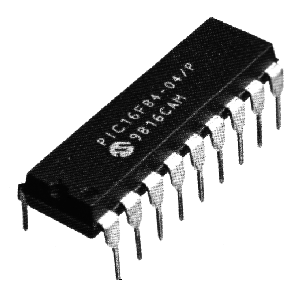
\includegraphics[width=2.0in] {Images/pic-chip.png}
        \caption{PIC - circuitstoday.com}
        \label{PIC}
\end{figure}

\item Arduino
\\An open source hardware board that is cheap but not as cheap as a PIC.  These are very popular among hobbyists due to them being very easy to use and having a vast collection of community written libraries to interface with all different types of hardware.
\\Arduino uses C or C++ programming language for development, this can be a good thing due to the fact that it provides the programmer with a large amount of control over exactly how the program runs but is more complex to use than some other languages such as python or java which handle a large amount of the low level operations for the developer.
\begin{figure}[H]
\centering
        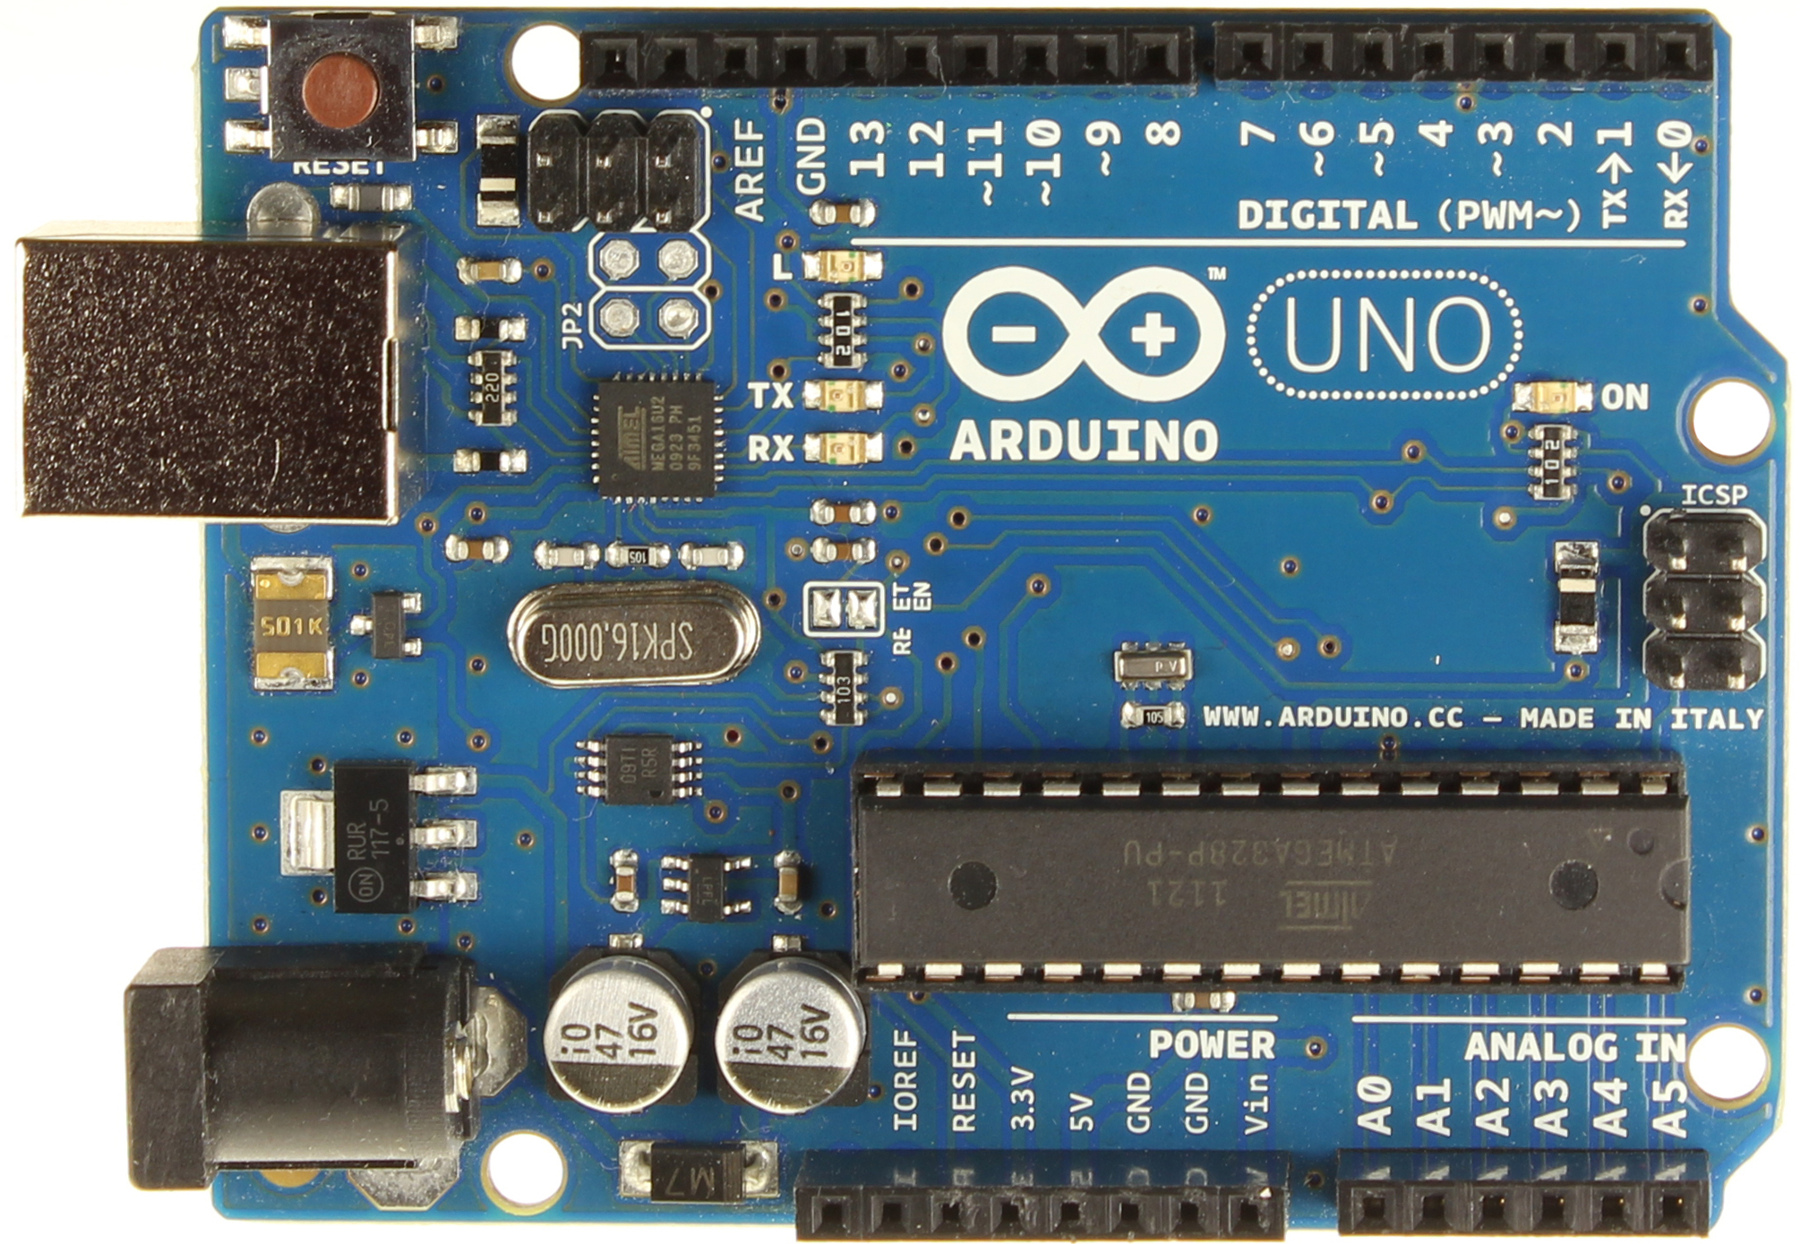
\includegraphics[width=2.0in] {Images/arduinouno-r3.jpg}
        \caption{Arduino arduino.cc}
        \label{Arduino}
\end{figure}

\item Netduino
\\This is also an open source electronics prototyping platform but instead of being based on C and C++ it is based on the .Net Micro Framework which is Microsoft's version of an embedded framework.  This could be useful to somebody who is very familiar with a .NET language such as C\#.  The main disadvantage is that this framework requires a faster processor to run and as such requires more power to operate making this option have higher overheads on power and processing than the PIC and Arduino alternatives.
\\These boards also cost more than the Arduino and PIC, and have much less community support.
\begin{figure}[H]
\centering
        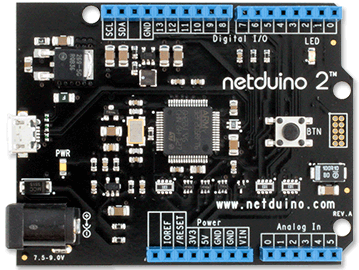
\includegraphics[width=2.0in] {Images/netduino.png}
        \caption{Netduino - netduino.com}
        \label{Netduino}
\end{figure}

\item Motherboard
\\A small motherboard that can be found in a home computer or a netbook/laptop.  These have the widest variety of applications.  It can support most operating systems and programming languages but come at the hefty price of power consumption.  Compared to microcontrollers, a full motherboard draws a very large amount of power to run.  Also they take far longer to power on due to running an operating system, unlike microcontrollers that have the code compiled down and run directly on the hardware itself.  This can also be done with these larger boards but is far more complex to do and is out of the scope of this project.
\\The cost of such boards is also very high as they are far more complex pieces of electronics.
\begin{figure}[H]
\centering
        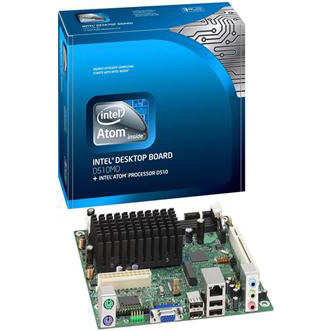
\includegraphics[width=2.0in] {Images/atom.jpg}
        \caption{Atom Motherboard - intel.co.uk}
        \label{Atom Motherboard}
\end{figure}
\item Raspberry Pi
\\The Raspberry Pi is a credit card sized computer that is an embedded platform for Linux and various other operating systems.  It is very cheap and runs much faster than most microcontrollers.  It does also have the downside of long startup times due to running a full desktop style operating system on such a compact board.  This could also be compiled to run directly on the ARM processor this board uses but is also out of the scope of this project.  Unlike normal motherboards this little board has some GPIO (general purpose input output) pins for interacting directly with various pieces of hardware like the microcontrollers do.
\begin{figure}[H]
\centering
        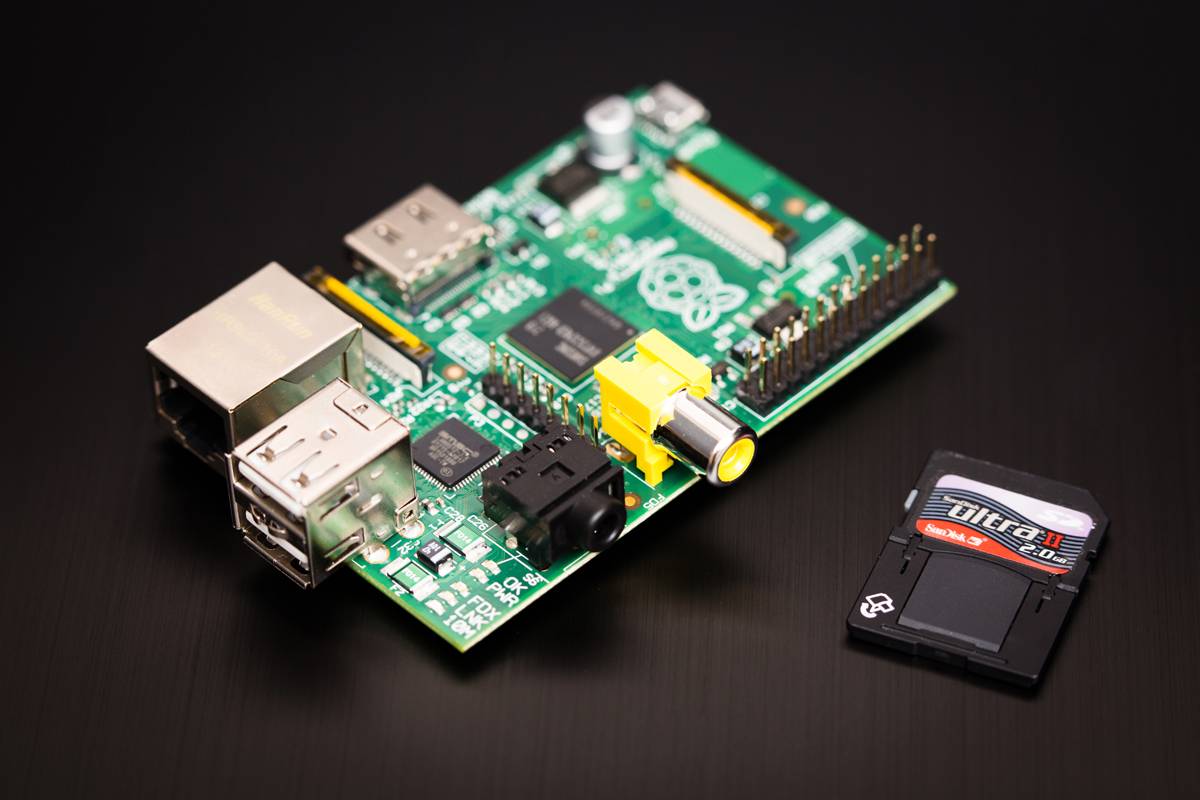
\includegraphics[width=2.0in] {Images/rpi.jpeg}
        \caption{Raspberry Pi - raspberrypi.org}
        \label{Raspberry Pi}
\end{figure}

\end{itemize}

\subsection{Power Source}
As this robot is intended to move around freely the power source should be:
\begin{enumerate}
\item Unhindered by power and data cables, the power source cannot be supplied by a wall power outlet, it has to be self contained.  This means it will have to be a battery.
\item The battery will have to be several cells or a single high output cell due to the size of motors intended.
\item It will need as many Amp hours as possible for longer run times.  This could be achieved with several cells linked together in series (end to end) to increase voltage and/or link more together in parallel (side by side) to increase amp hours (runtime).
\item It will have to be small enough to fit on the robot.
\item It should be light as to not increase the load on the drive system too much.
\end{enumerate}
The possible options are:
\begin{itemize}
\item Lithium Polymer
\\LiPo batteries come in up to 11.2 volt packages, which is not quite high enough for some higher voltage motors which I may be using such as the high end steppers.  These batteries are much lighter than some other alternatives and are common in embedded devices.  The amp hour ratings of these batteries can range from 100 milliamp hours to around typically 6 amp hours in the size packages that would be suitable for a small robot.
\begin{figure}[H]
\centering
        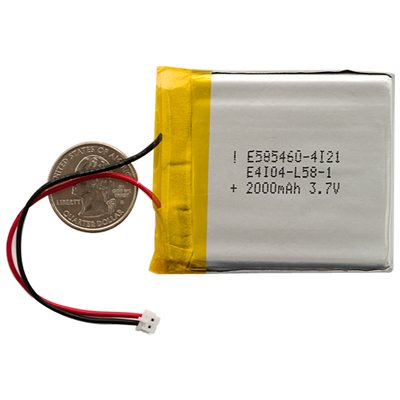
\includegraphics[width=2.0in] {Images/lipo-front.jpg}
        \caption{Lithium Polymer Battery - robotshop.com}
        \label{Lithium Polymer Battery}
\end{figure}

\item Lead Acid
\\A lead acid battery is a choice with a high output.  A single battery can output 12 volts and can be found in high amp hour packages such as 1 - 40amp hours compared to the lithium alternatives which are around 0.1 - 6 amp hours.  Due to already needing a high power motor for the chassis, a higher weight battery is not too much of an issue and provides the benefit of the higher power output to drive the more power hungry motors.
\begin{figure}[H]
\centering
        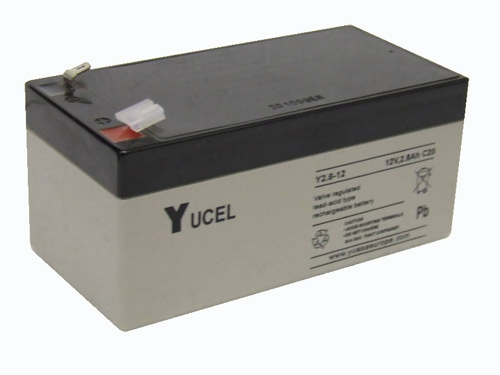
\includegraphics[width=2.0in] {Images/lead-acid.jpg}
        \caption{Lead Acid Battery - kestrelelectricalsupplies.co.uk}
        \label{Lead Acid Battery}
\end{figure}
\end{itemize}
\subsection{Wheels}
As I have chosen a wheeled solution for the drive system of the robot the wheels supporting it must be appropriate.
\\The perfect wheels would be:
\begin{enumerate}
\item Made of extremely light materials thus being easier to turn.
\item To be very strong to support all of the weight of the robot on them.
\item To have a high level of traction as not to slip on the environment it may be traversing.
\item As cheap as possible to keep overall costs to a minimum.
\item Be easy to mount to the drive shaft of the motors being used to move the wheels.
\end{enumerate}
\begin{itemize}
\item Off Road
\\Having chosen to use stepper motors for the reason of increased accuracy over the less precise DC motors it would be a bad idea to go for wheels which have insufficient traction and as such off road style wheels which have a wide and deep tread with spikes for additional grip would be a suitable solution.
\\These wheels measure 120mm in diameter and 60mm wide which results in it being harder to turn and will require a stronger motor to move.
\begin{figure}[H]
\centering
        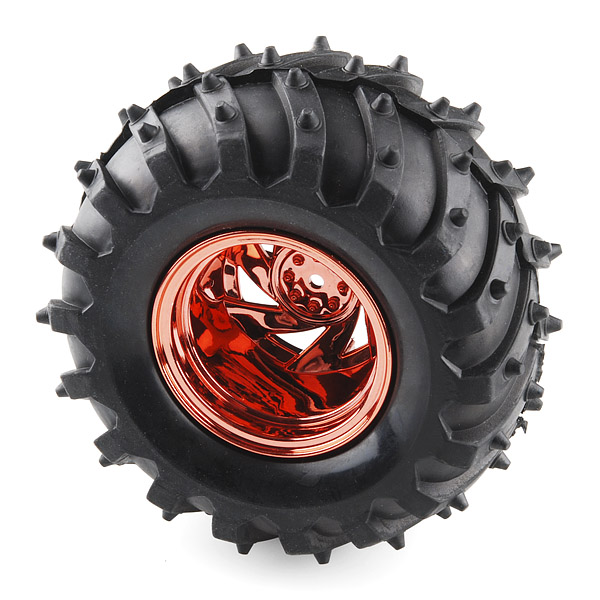
\includegraphics[width=3.0in]  {Images/wheel-offroad.jpg}
        \caption{Offroad Wheel - sparkfun.com}
        \label{Offroad Wheel}
\end{figure}

\item Colson Wheel
\\These come in sizes ranging from four inches to twelve inches in diameter with a tread width of between two and three inches.  They have a rubber exterior for grip with an iron core for mounting.  They are shock absorbent but this should not be an issue for this project due to the slow speeds that it is intended to be moving at.  The iron core makes these wheels very heavy weighing around four pounds for the smaller wheel and up to sixteen pounds for the larger versions.
\begin{figure}[H]
\centering
        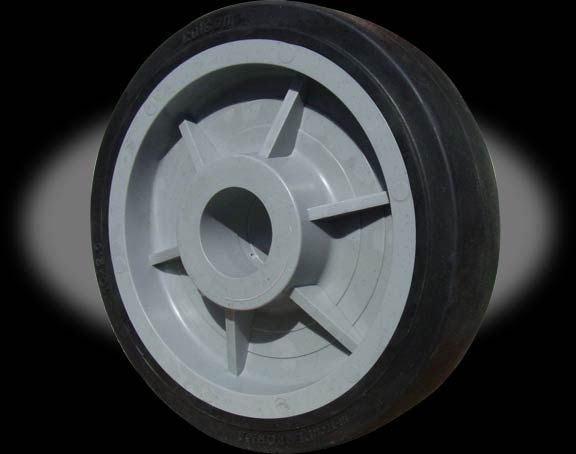
\includegraphics[width=3.0in]  {Images/colson.jpg}
        \caption{Colson Wheel - colsoncaster.com}
        \label{Colson Wheel}
\end{figure}
\item Omni Wheel
\\These wheels have been briefly described in the four wheeled drive system section but here I will go into more detail.
\\They have less grip then other wheel types due to the rollers all around the wheel.  Their primary advantage is that when two or more are used in conjunction with each other and are rotated in different directions they can move whatever device they are mounted to directly sideways, this is going against the way the wheels are actually turning.  This feature of the omni wheels is a major advantage if the robot gets stuck in a tight space that it cannot turn to get out of or even just a tight turn that it's normal turning circle is not sufficient to traverse.
\begin{figure}[H]
\centering
        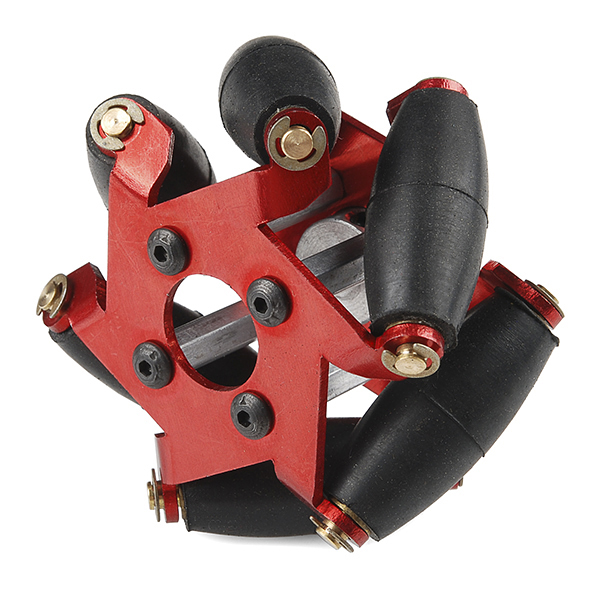
\includegraphics[width=3.0in] {Images/mechanum.jpg}
        \caption{Omni Wheel - sparkfun.com}
        \label{Omni Wheel}
\end{figure}

\end{itemize}
\section{Feedback Interface}
While operating the robot, if there is any unexpected behaviour it would be nice to have some form of interface to see what the robot thinks the environment looks like.
\\An ideal solution for this should conform to the following guidelines:
\begin{enumerate}
\item There cannot be any cables trailing from the robot to the feedback device because you do not want to have to follow the robot around it's environment just to be able to read what it thinks it is seeing, so a wireless solution would be good.
\item Be lightweight so that carrying it is not a nuisance.
\item Low power consumption so that it does not need to be near a power source all the time.  Having a run time the same as or longer than the robot itself would be ideal.
\item Easy to read display which is also low power.
\item Intuitive user interface so that it is very easy to use and enables the user to just use it without any instruction.
\end{enumerate}
All that is needed is a small microcontroller as learned from the previous sections that these are low powered, easy to use and have support for various different pieces of hardware.
\\Lithium ion batteries are a good fit for this sort of device due to their low weight, low voltage and small size.
\\A small display is needed.
\begin{itemize}
\item Liquid Crystal Display
\\These are low powered easy to use devices for displaying information.  They are used in everyday machines such as a digital display on an oven or microwave, the screen on a calculator or a vending machine even the screens used in mobile telephones.  These screens are very cheap and easily available in all sorts of types and sizes.
\begin{figure}[H]
\centering
        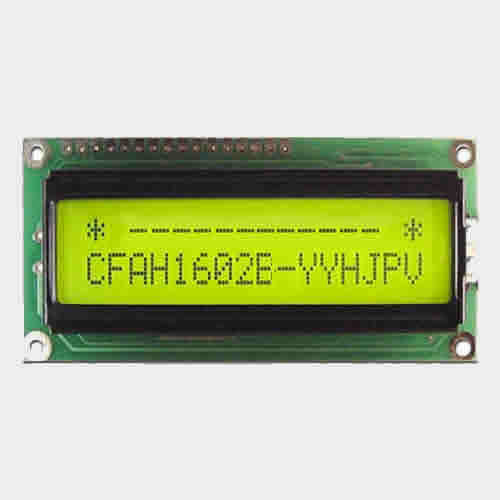
\includegraphics[width=2.0in] {Images/lcd.jpg}
        \caption{Liquid Crystal Display - coolcomponents.co.uk}
        \label{Liquid Crystal Display}
\end{figure}
\item E-Ink Display
These displays are unique in that they only use power to change what they are displaying, once the display has changed it used no more energy to keep the screen displaying it's current image.  The main downside to these is getting hold of one that has not been removed from another device such as an e-reader.  Some of these displays are also flexible and could be used to wrap around the wrist as a type of watch display.  They are also very expensive for a simple display but the power consumption aspect makes them a very attractive option for this type of device.
\begin{figure}[H]
\centering
        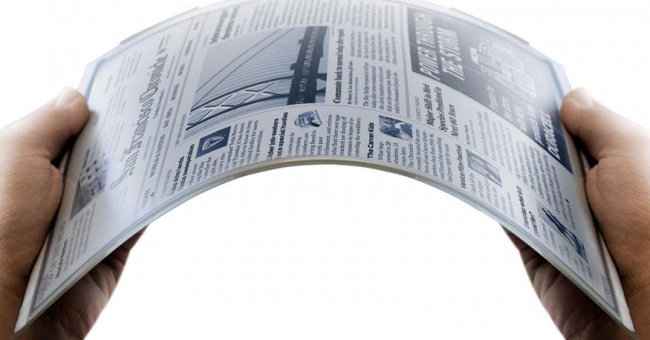
\includegraphics[width=4.0in] {Images/e-ink-display.png}
        \caption{E-Ink Display - dataprotectioncenter.com}
        \label{E-Ink Display}
\end{figure}
\end{itemize}
A wireless module of some description will be needed to transmit the information from the robot to the feedback device.  This device should ideally conform to these guidelines:
\begin{enumerate}
\item Have as much range as possible so that no matter how far away the robot goes it can still receive the information from it.
\item Be able to transmit through any material so that no matter what obstacles get between the robot and the feedback device it can still receive information.
\item Consume as little amount of power as possible to increase the run time of the device.
\item Be physically small to keep the size of the device as small as possible.
\item Be as light as possible to keep the overall device weight to a minimum for comfort as the user may be holding it for prolonged periods of time.
\end{enumerate}
The options for this type of component are:
\begin{itemize}
\item Wifi
\\This is the most common wireless medium for transmitting large amounts of data.  It has some low powered modules with a consumption rate of only 100 milliwatts and this low power module can transmit data at 1Mbps (mega bits per second).  The downside is that these low power versions are expensive costing around fifty dollars a piece.
\begin{figure}[H]
\centering
        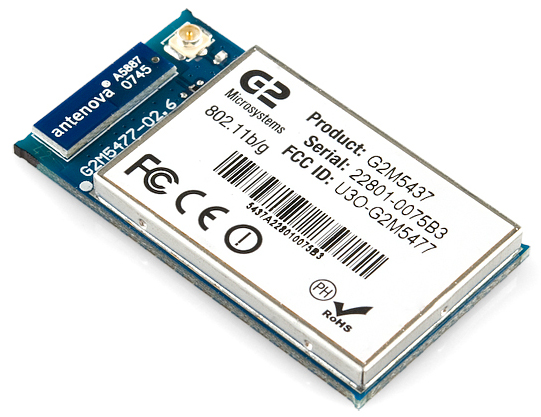
\includegraphics[width=2.0in] {Images/wifi-module.jpg}
        \caption{Wifi Module - antenova-m2m.com}
        \label{Wifi Module}
\end{figure}
If a USB connection is available with a host that has the appropriate drivers to run a USB wifi module then a cheaper version is available at around fifteen dollars but these have a much higher processing overhead for any device that is capable of using such a module which in turn uses more power.  The module itself is still around 100-500 milliwatts of power usage.
\begin{figure}[H]
\centering
        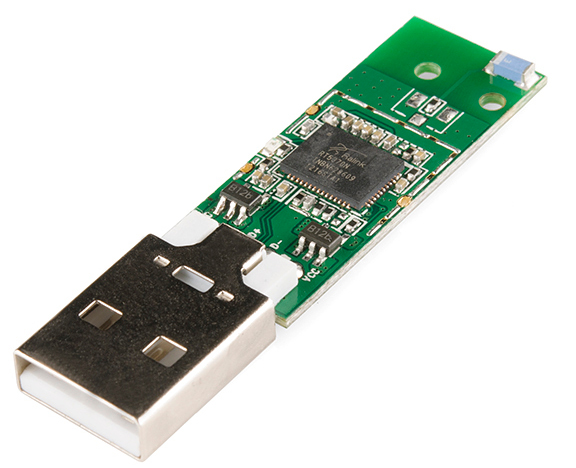
\includegraphics[width=2.0in] {Images/usb-wifi.jpg}
        \caption{USB Wifi - sparkfun.com}
        \label{Usb Wifi}
\end{figure}
Both of the Wifi module types have a maximum range of around one hundred meters.

\item Bluetooth
This type of communication is commonly using in mobile telephones to enable such things as hands free calls in an automobile.  Low power Bluetooth units that transmit data at around 1200 bits per second typically use only 24 milliwatts of power in doing so.  This is much lower than the low power version of wifi but it has severe range limitations of only being reliable within 10-20 meters.  The Bluetooth modules available for use in hobbyist projects such as this are rather pricey costing around forty dollars each.
\begin{figure}[H]
\centering
        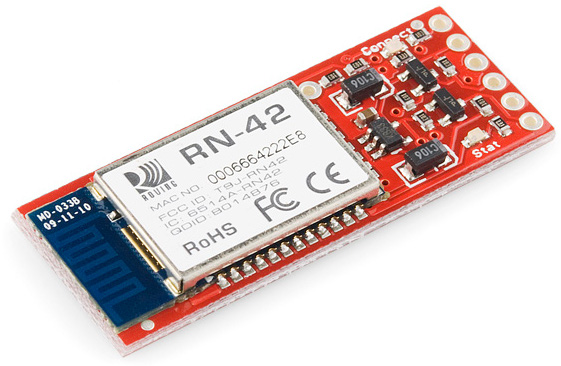
\includegraphics[width=2.0in] {Images/bluetooth.jpg}
        \caption{Bluetooth Module - sparkfun.com}
        \label{Bluetooth Module}
\end{figure}
\item Zigbee
These little wireless radios are perfect for small, low powered wireless projects.  They run on as little as 3.3 volts with an output of 1 milliwatt.  The downside is that it's data transfer rate is only around 250 killobits per second, just a quarter of the embedded wifi module.  The zigbee module more than makes up for the lack of data transfer with its increased range of up to 100 meters.  These are also one of the cheaper options costing around twenty dollars each.  These such modules are called xbee which is just an implementation of the zigbee protocol which is typically used for mesh networking but still works for single point to point communications.
\begin{figure}[H]
\centering
        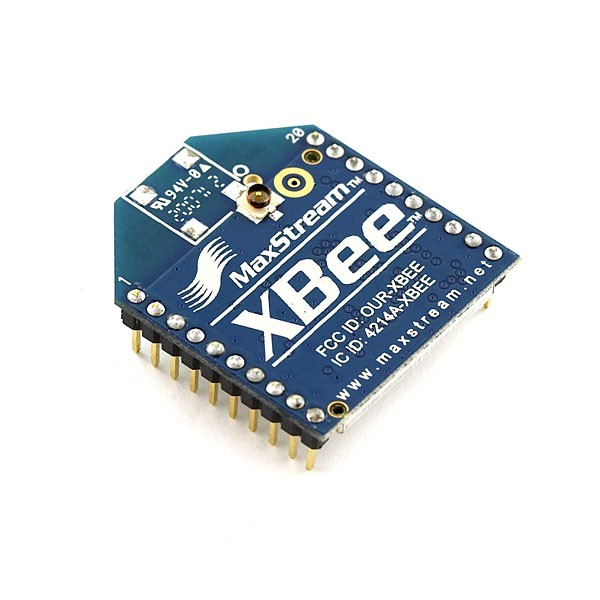
\includegraphics[width=3.0in] {Images/xbee.jpg}
        \caption{Xbee Module - sparkfun.com}
        \label{Xbee Module}
\end{figure}

\end{itemize}
An Arduino Fio is a good fit as it is small, low powered, has both lithium polymer battery socket and an xbee wireless module socket built in making it the obvious choice for this type of device as most of the connection work has been done already just leaving the screen and a user input method to be added.
\\A small LCD (liquid crystal display) can be connected to the Arduino to display information it receives over the integrated xbee socket.
\\A user input interface can be added by using some small push buttons and wiring them to some of the input pins provided on the Arduino Fio.


\chapter{Implementation}

%The implementation should look at any issues you encountered as you tried to implement your design. During the work, you might have found that elements of your design were unnecessary or overly complex, perhaps third party libraries were available that simplified some of the functions that you intended to implement. If things were easier in some areas, then how did you adapt your project to take account of your findings?

%It is more likely that things were more complex than you first thought. In particular, were there any problems or difficulties that you found during implementation that you had to address? Did such problems simply delay you or were they more significant? Your implementation might well be described in the same chapter as Problems (see below).

\section{Prototype}
It is a good idea to first build a basic prototype.  Building a prototype will quickly highlight the main flaws in the initial design.  This is not the same as the intended final version and in this case is not even the same materials as I have chosen.  It does however conform the basic design but is made from much cheaper sourced components.  I already had an Arduino Uno (the basic prototyping model) from my interest int he technology before I attended university, so this was an easy component to get ym hands on quickly and is perfect for a prototype.  I had no chassis built or any materials to make one so I found a cheap and easy to assemble one online at a hobbyist electronics retailer.  This kit also included some very small DC motors with gearboxes and wheels, very convenient little package.  The Arduino alonge with the chassis kit and a small infrared sensors, a 9 volt battery and some jumper wires and a ptorotype was put together in an afternoon.
\begin{figure}[h]
\centering
        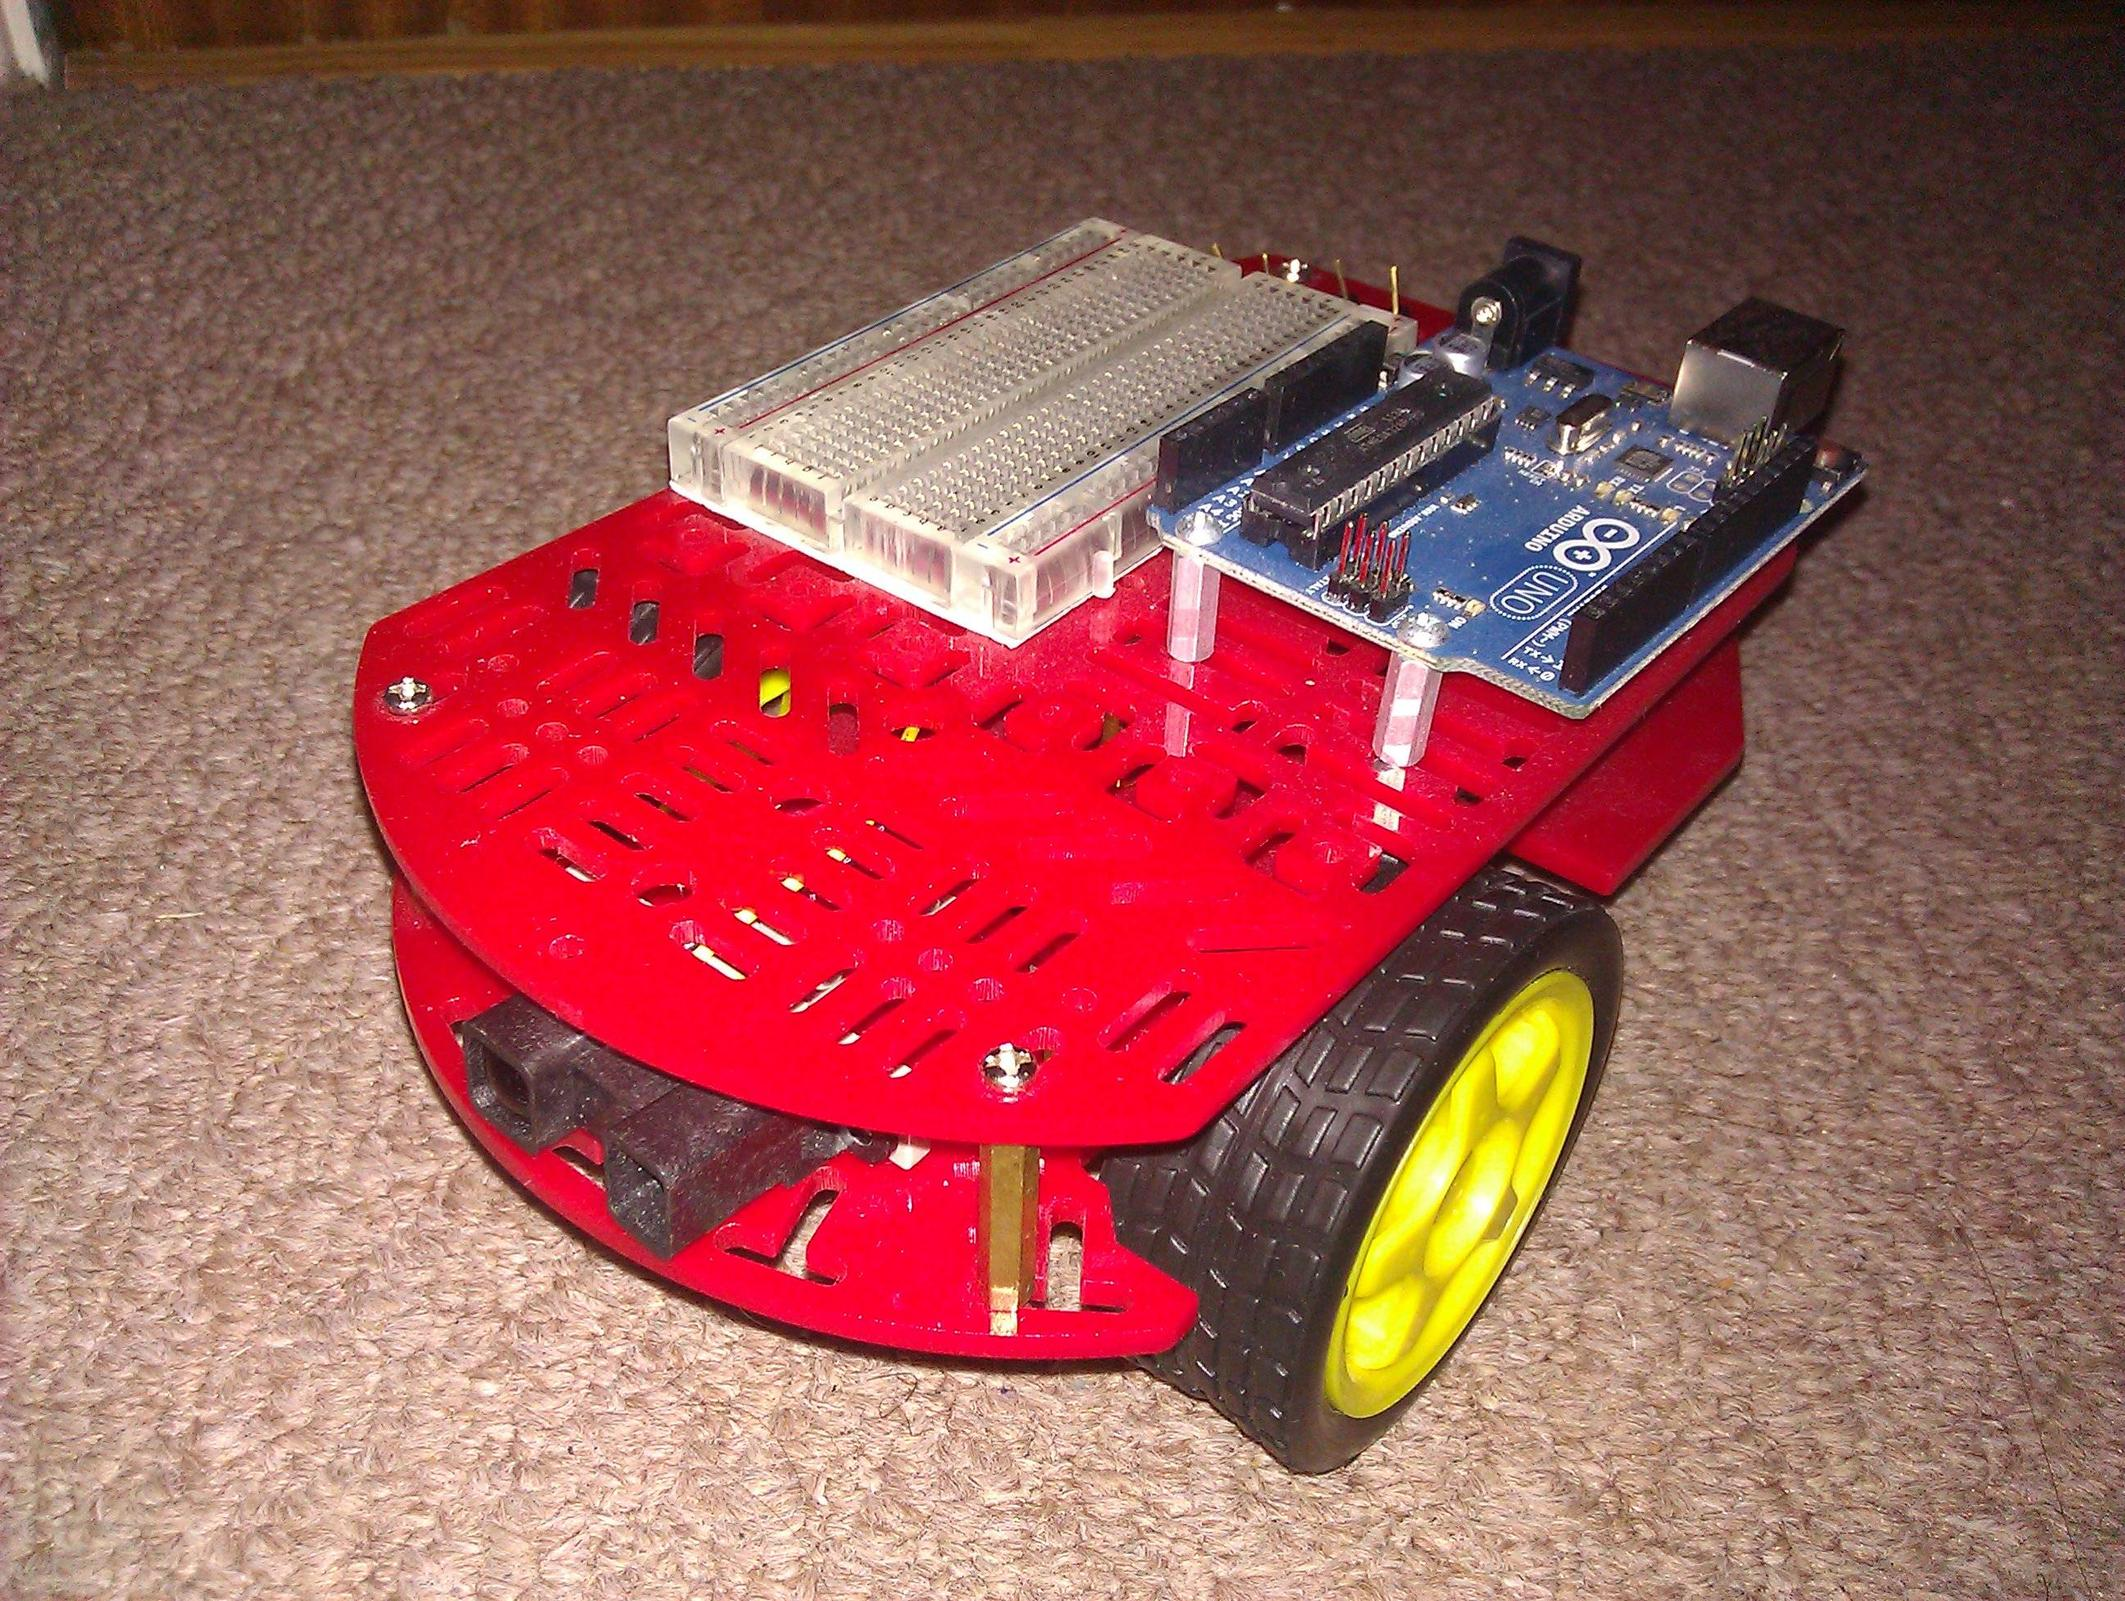
\includegraphics[width=3.0in] {Images/tria-mkI.jpg}
        \caption{Prototype mkI}
        \label{Prototype mkI}
\end{figure}

Wiring up the components was fairly easy due to there only being two motors and a single infrared sensor.  The sensor just has 3 pins, ground and possitive power pins as well as a signal pin.  This is basicly set up like a resistor, you supply power the the possitive pin, attach the ground to the ground of the system and just read the value comming back on the signal pin.  The difference between zero up to the amount of power being given to the sensor, in this case the datasheet specified 5 volts and that is what I supplied it with, gives an inidication of how far it is from an object.  With this sensor the higher value returned is actually how close the object is and the lower number indicates it is further away.  This is due to the fact that the reading recieved is indicating how intense the amount of infrared getting back to the sensor is.
\\The harder part of this was getting the motors to run safely.  The arduino I use for prototyping can only output a regulated voltage of 3.3 or 5 volts.  The motors supplied with the chassis kit do not run very well at this voltage and struggle to move on carpet.  As the supply I am using to power the Arduino is a 9 volt battery this was usfficient to run the motors at an acceptable level, the only problem is supplying this to both the Arduino and the motors.  As the microcontroller is needed to control when and how fast the motors are to turn, simply wiring the power supply directly to the motors is a bad idea as they will just spin constantly due to always having power.
\begin{figure}[h]
\centering
        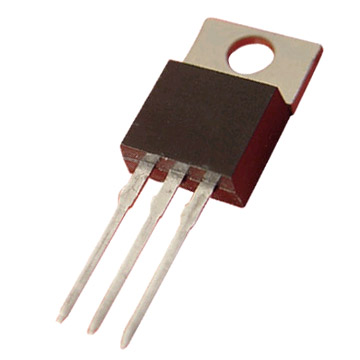
\includegraphics[width=2.0in] {Images/transistor.jpg}
        \caption{Transistor - zmescience.com}
        \label{Transistor}
\end{figure}

This could be solved using a transistor (a semi-conductor device used to switch electrical signals) by suppling it with the higher voltage, connecting it to the motor and when a signal voltage from the Arduino is recieved it switches to the higher voltage allowing the motor to turn.  This is a very handy little component which is at the core of modern day electronics, but to use it in this fashion would need a lot more complicated circuitry as to ensure that this higher voltage does not damage other components in the circuit.  Another solution would be to use a chip known as a h-bridge.
\\This chip also acts like a switch but with the addition that it can change the currents direction meaning that you can not only control when the motor is on or off but also the direction it turns without additional complex circuitry.
\begin{figure}[h]
\centering
	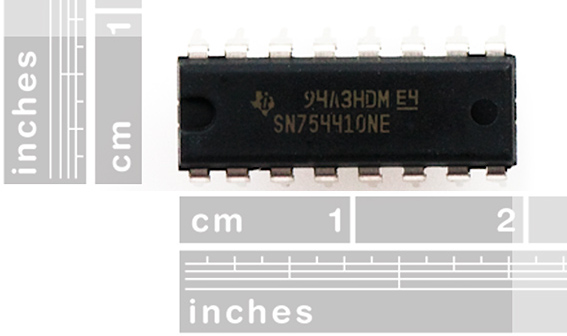
\includegraphics[width=2.0in]  {Images/h-bridge.jpg}
	\caption{H-Bridge - sparkfun.com}
	\label{H-Bridge}
\end{figure}
The h-bridge chip also has its issues, as it generates heat when high currents are passed through it so if the motors are working hard more current with be drawn and the more heat the chip will generate and possibly burn out.  There is again the issue of having no protection for the rest of the circuit.  An option that would solve this issue is a full motor driver board but the cost if these is many times the cost of the components to make the circuits myself.  For example a h-bridge chip an assortment of diodes, capacitors, resistors and transistors costs around \pounds5 while a fully built board costs around \pounds20-30.
\begin{figure}[h]
\centering
        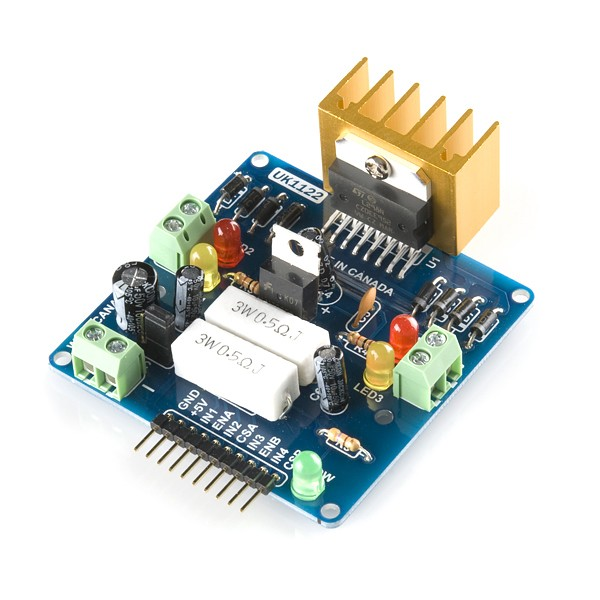
\includegraphics[width=2.0in]  {Images/motor-driver.jpg}
        \caption{Motor Driver - sparkfun.com}
        \label{Motor Driver}
\end{figure}
I decided to build a simple motor driver using the h-bridge chips, effective for a simple prototype.
\\With only a single infrared sensor the only logical place to mount it would be to have it facing directly forwards.  After writing the code to control the motors and process readings taken from the front mounted sensor the logic to test the concept is very simple.  Just check if there is something close in front and if there is just turn and check again, if there is not just keep moving forwards.
The logic looks like this:
\begin{figure}[h]
\begin{lstlisting}[basicstyle=\ttfamily]
if(sensor_range < value)
{
	motors.turn.right(45);
}else
{
	motors.move.forward(1);
}
\end{lstlisting}
\caption{Prototype Code Exert}
\label{Prototype Code Exert}
\end{figure}
This seems to work quite well, it does drive forwards and it does turn when an object comes in range of the infrared sensor.  This is the desired behaviour but there is a problem.  If the robot turns away from one object and into another, if that second object is too close by the time it comes in front of the sensor then it can not be seen by the sensor.  The sensor that I have fitted to the prototype has a maximum range of 150cm, but it also has a minimum range of 20cm meaning that is blind to any object closer than this minimum range.
\\In the figure the red signifies the blind area of the sensor and the green is the visible area.  If the robot were to turn right to avoid the wall in front of it then it would colide with the other wall and not be able to detect it.
\begin{figure}[h]
\centering
        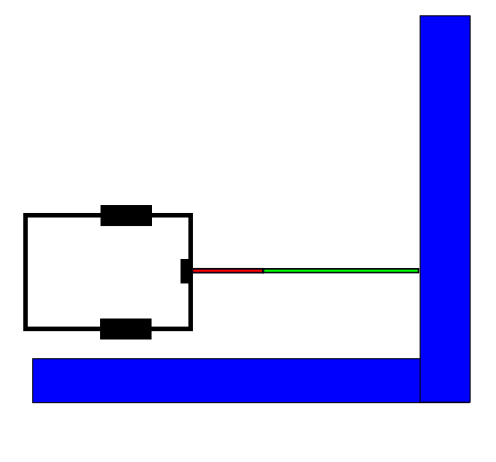
\includegraphics[width=3.0in]  {Images/ir-demo.png}
        \caption{Collision Illustration}
        \label{Collision Illustration}
\end{figure}
Another issue with the prototype robot is with the motors.  Even though I am supplying each motor with the same voltage they do not turn at the same speed, this is due to the lack of feedback with controlling them.  Also the fact that it is built from a very cheap kit is a probable reason for how uneven the speed of the motors is.  This all leads to the robot driving in a curve as opposed to the intended straight line, also contributing to the sensor problem of turning into an object putting it within the sensor blind spot.
\section{MK-I}
The next step is to build a version based on the design and using the things I have learnt from the prototype to improve it.
\\First thing to do it build a sturdy chassis for all the systems to be mounted onto.  I bought several sheets of aluminium to but cut into a similar shape as the small red plastic prototype.
\begin{figure}[h]
\centering
        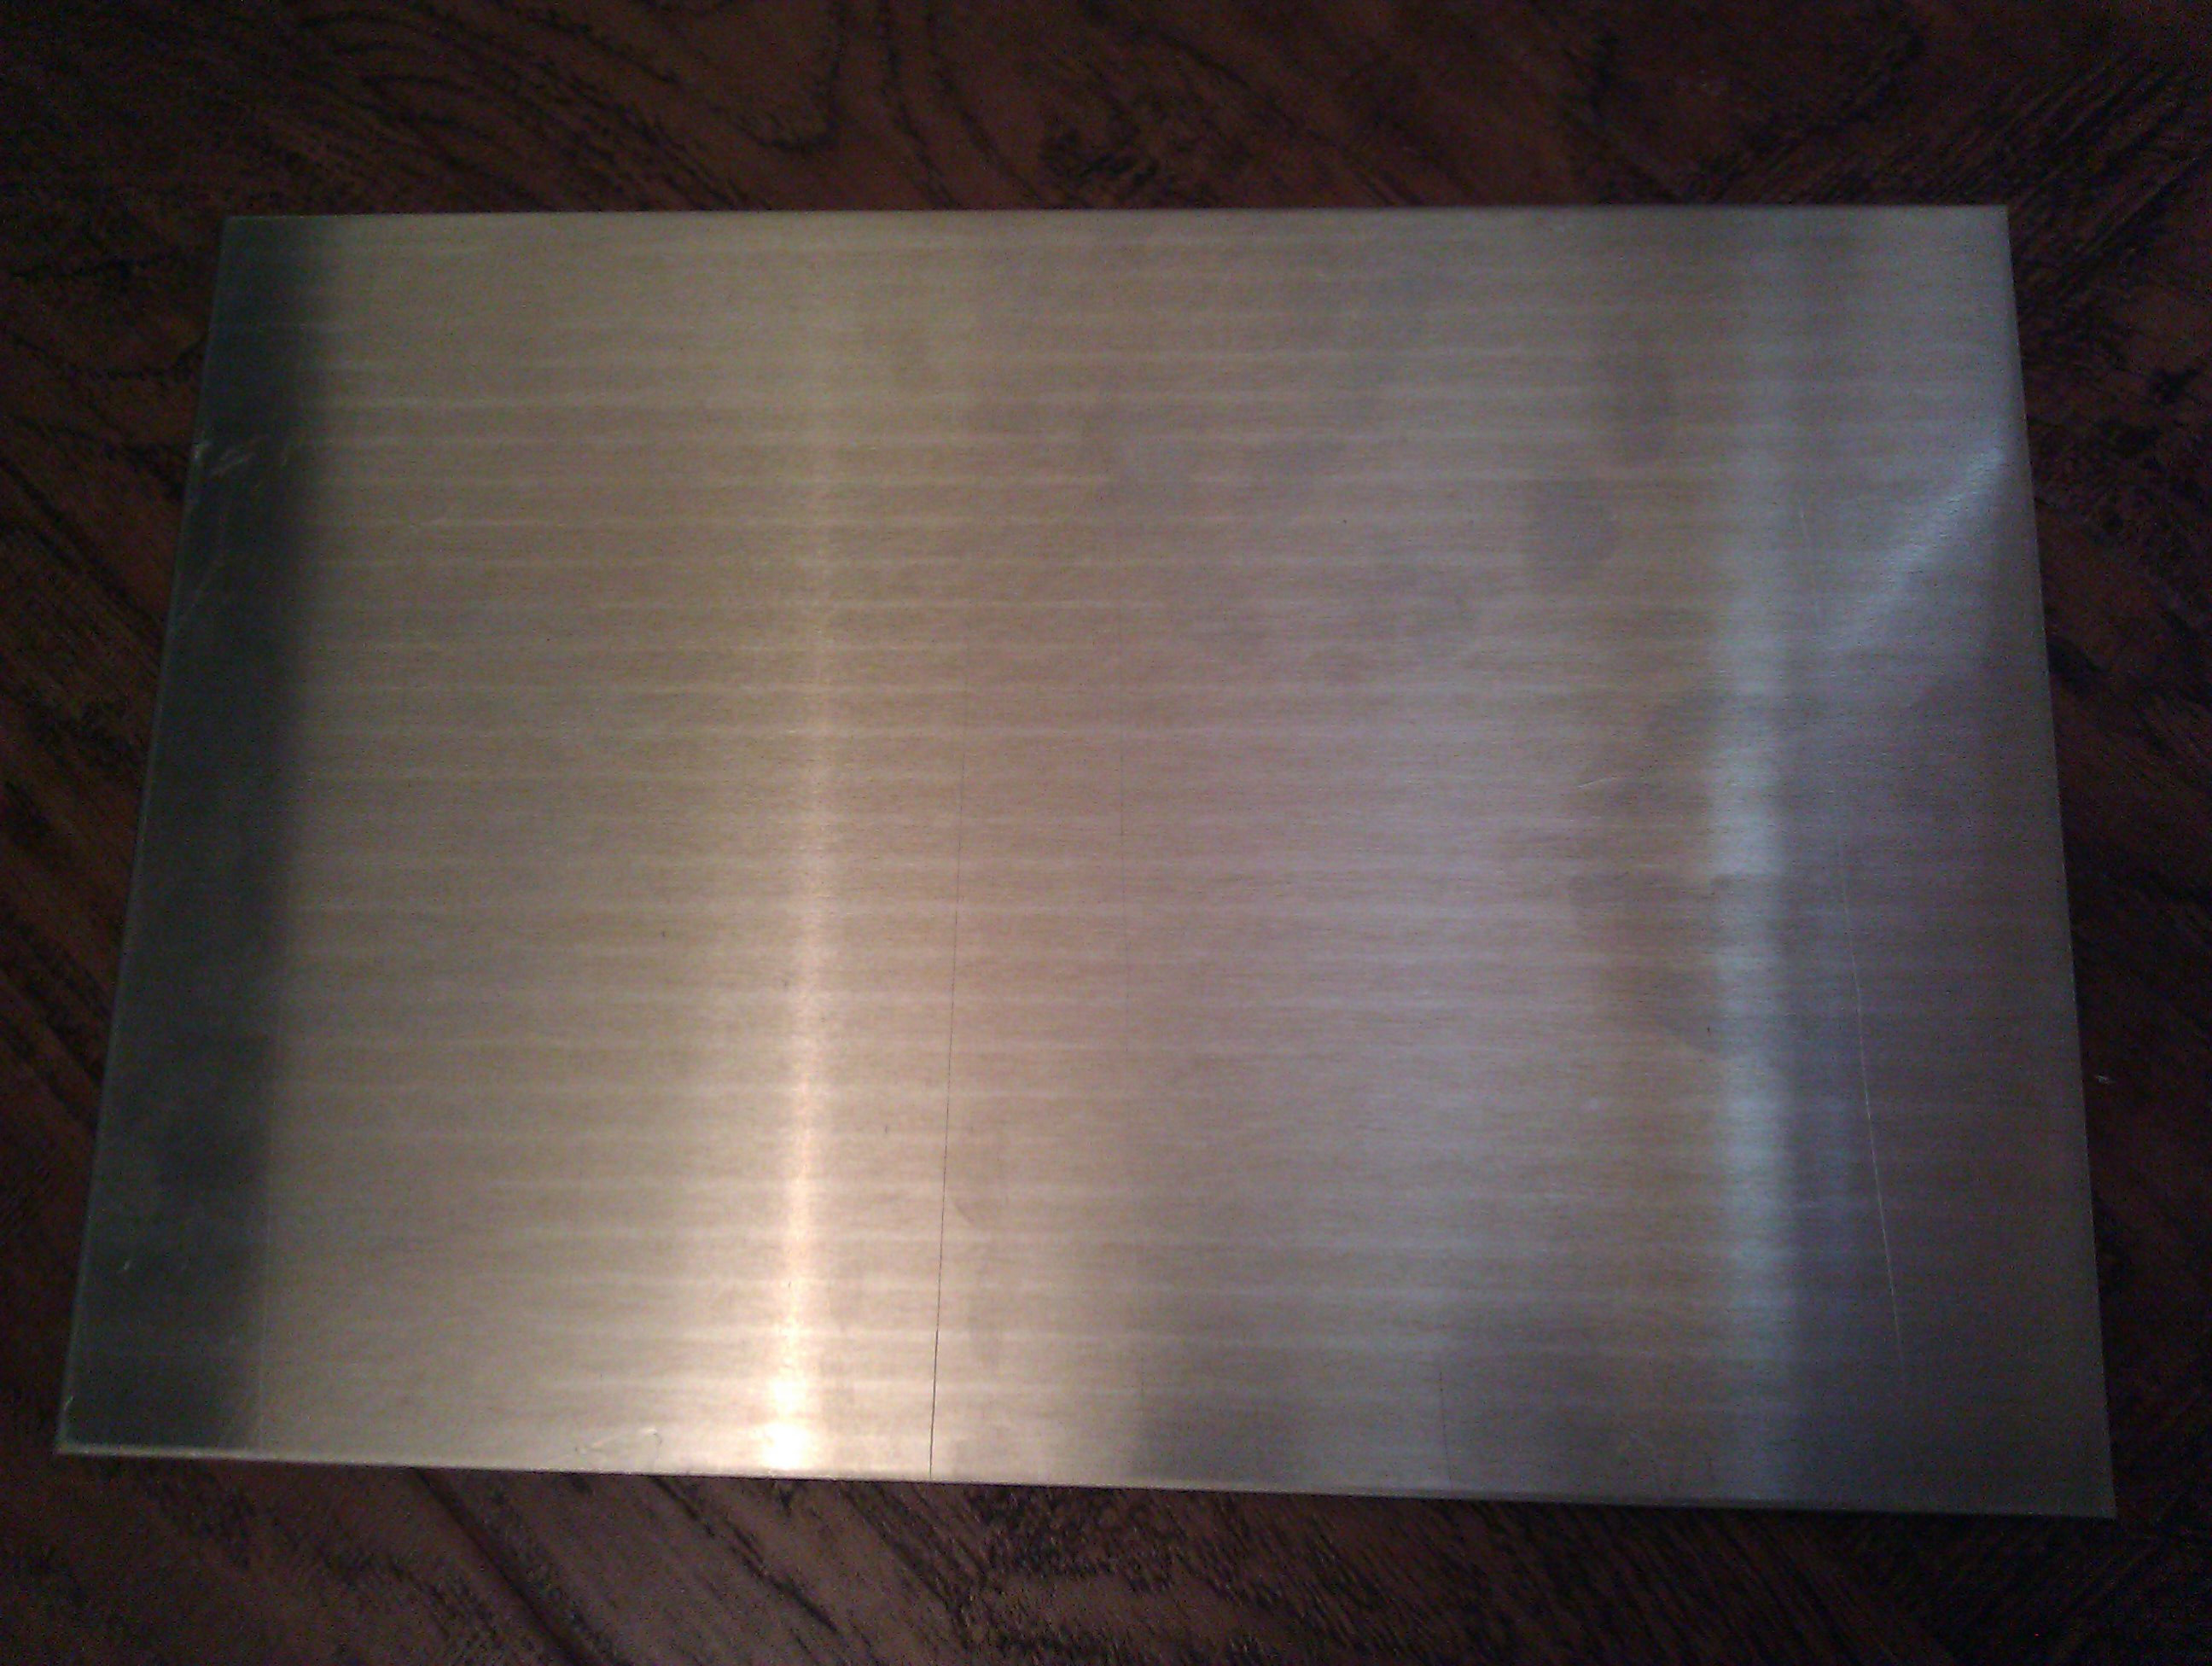
\includegraphics[width=3.0in]  {Images/alu-sheet-2.jpg}
        \caption{Aluminium Sheet}
        \label{Aluminium Sheet}
\end{figure}
I chose this shape mainly because of how much I liked working with said prototype but also because that a curved front seemed logical for mounting an array of sensors to.
\begin{figure}[h]
\centering
        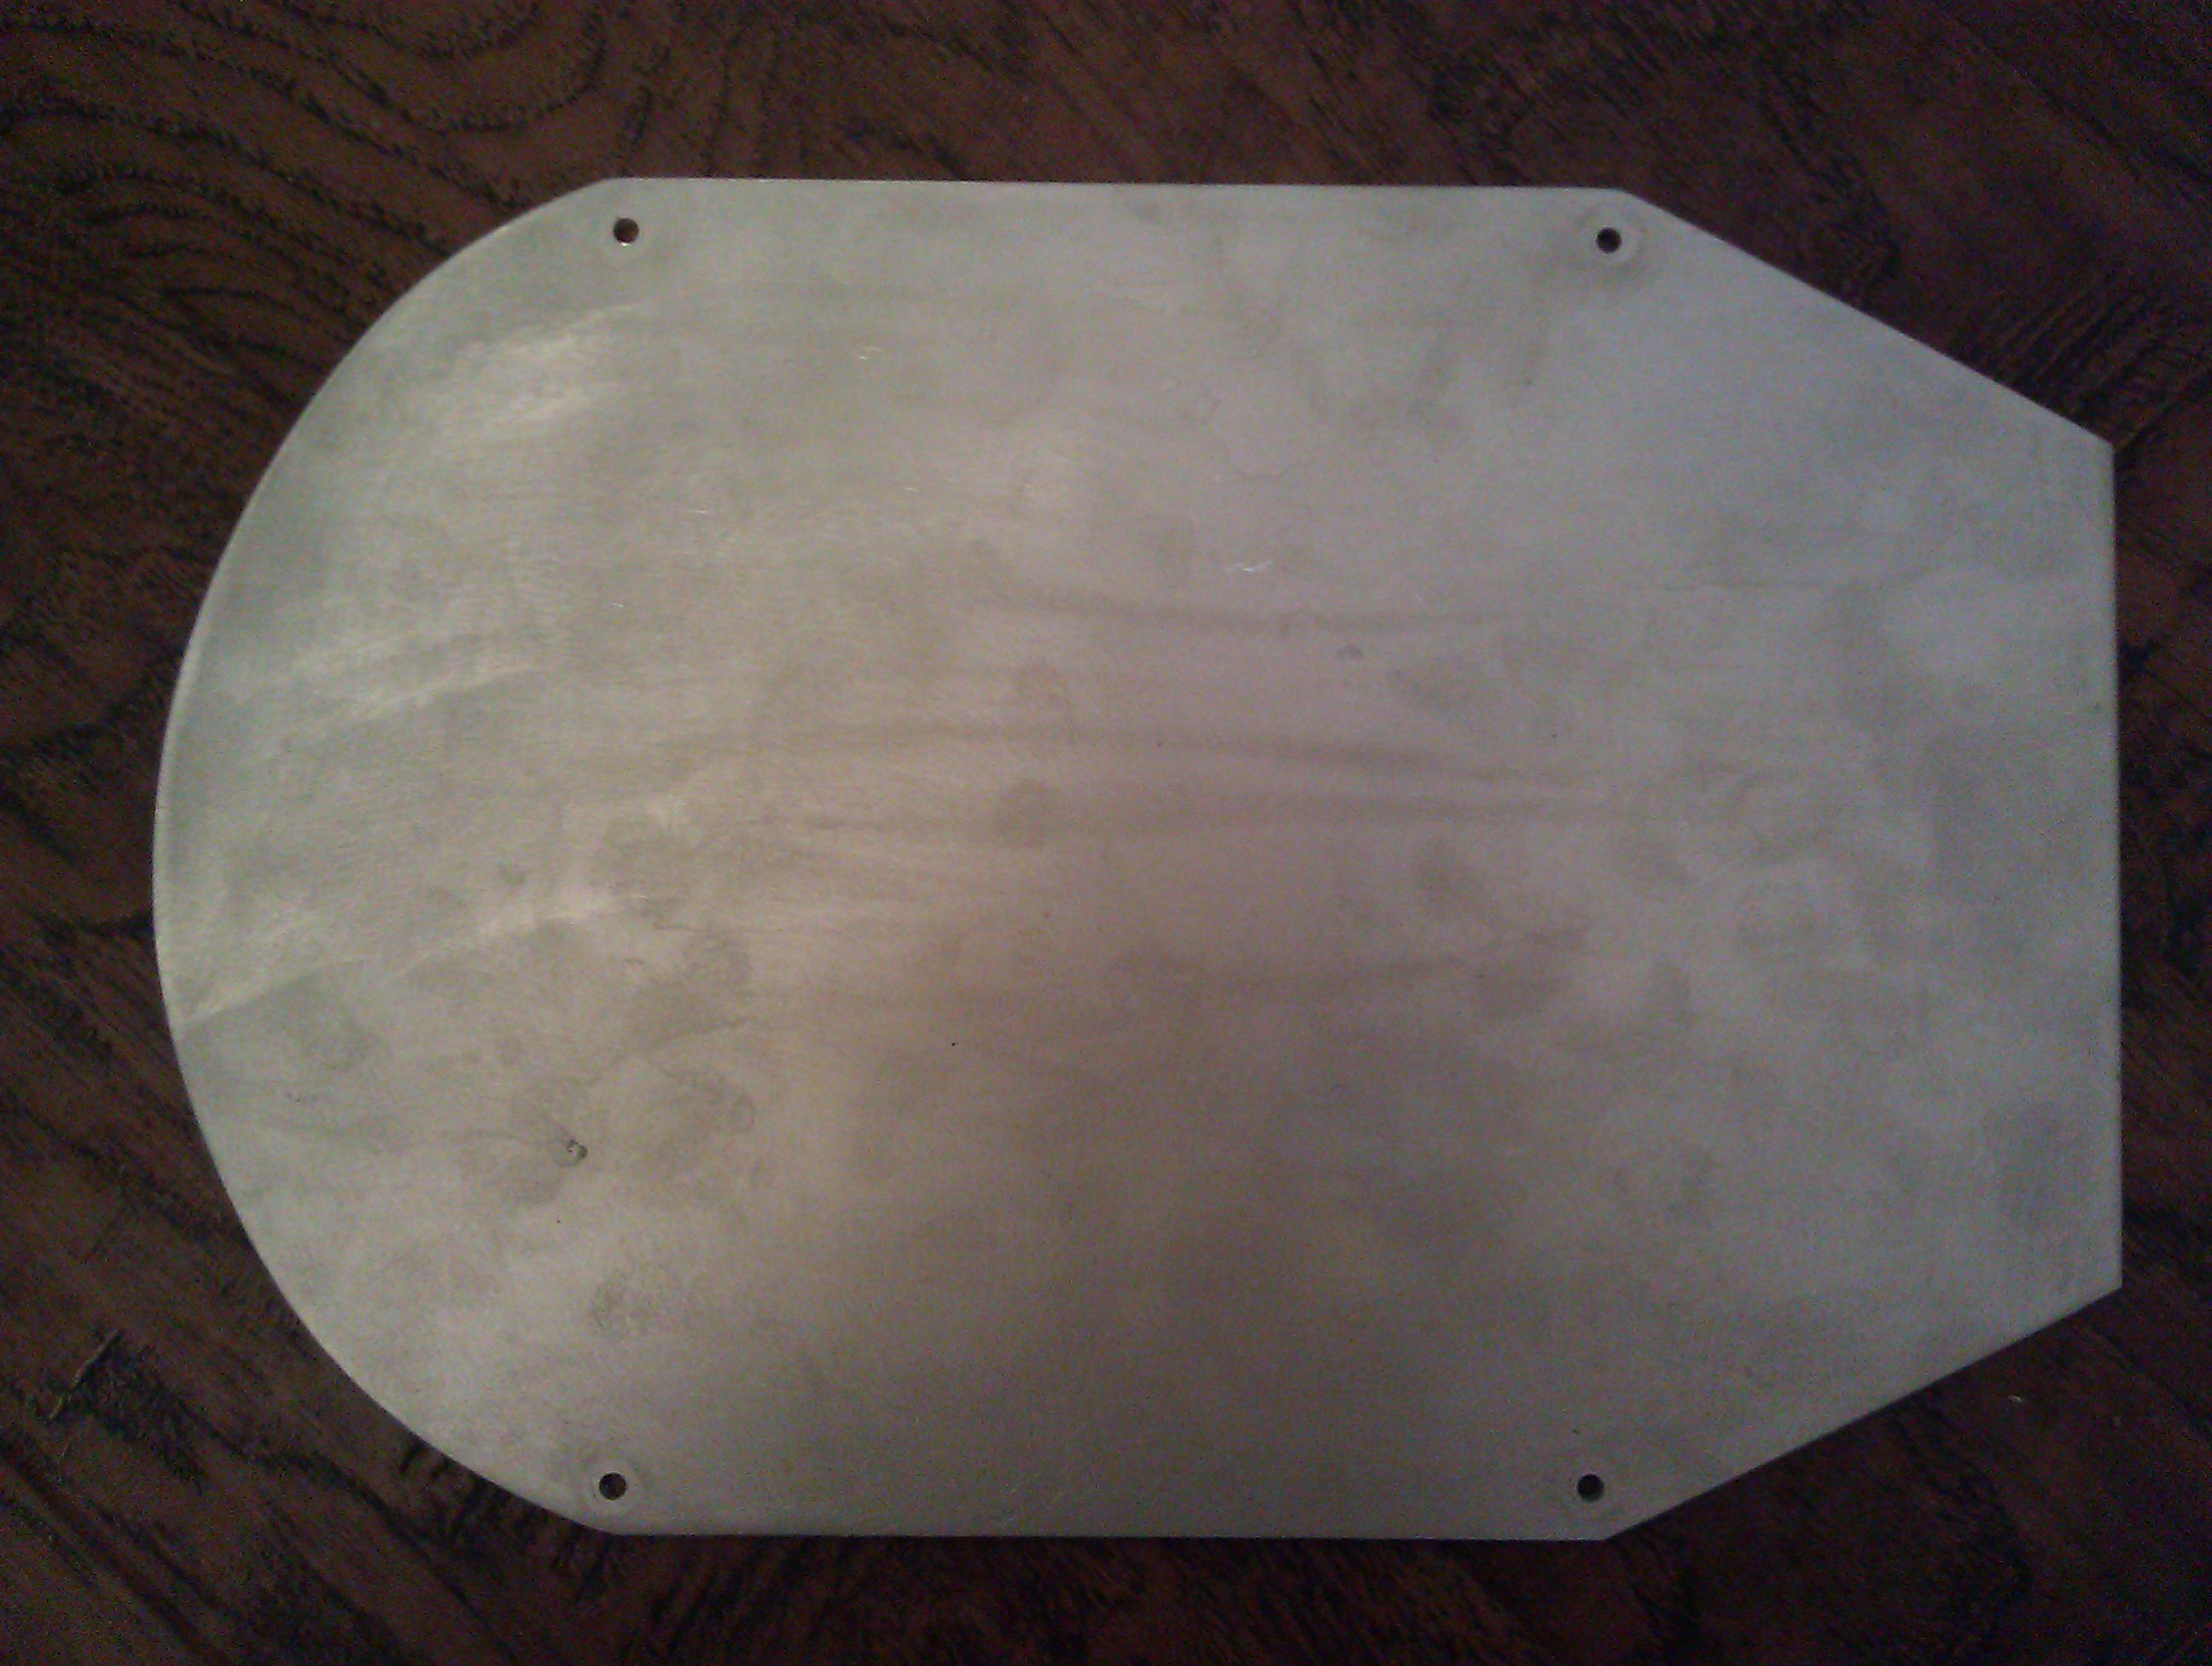
\includegraphics[width=3.0in]  {Images/alu-cut-2.jpg}
        \caption{Aluminium Sheet Cut}
        \label{Aluminium Sheet Cut}
\end{figure}
\\Next is to think about how to mount the motors to this aluminium base plate. After measuring the size of the stepper motors I bought to use as part of the robots drive system I also purchased a strip of aluminium to be cut and shaped into a motor mount to be attached on the underside of the baseplate.
\begin{figure}[h]
\centering
        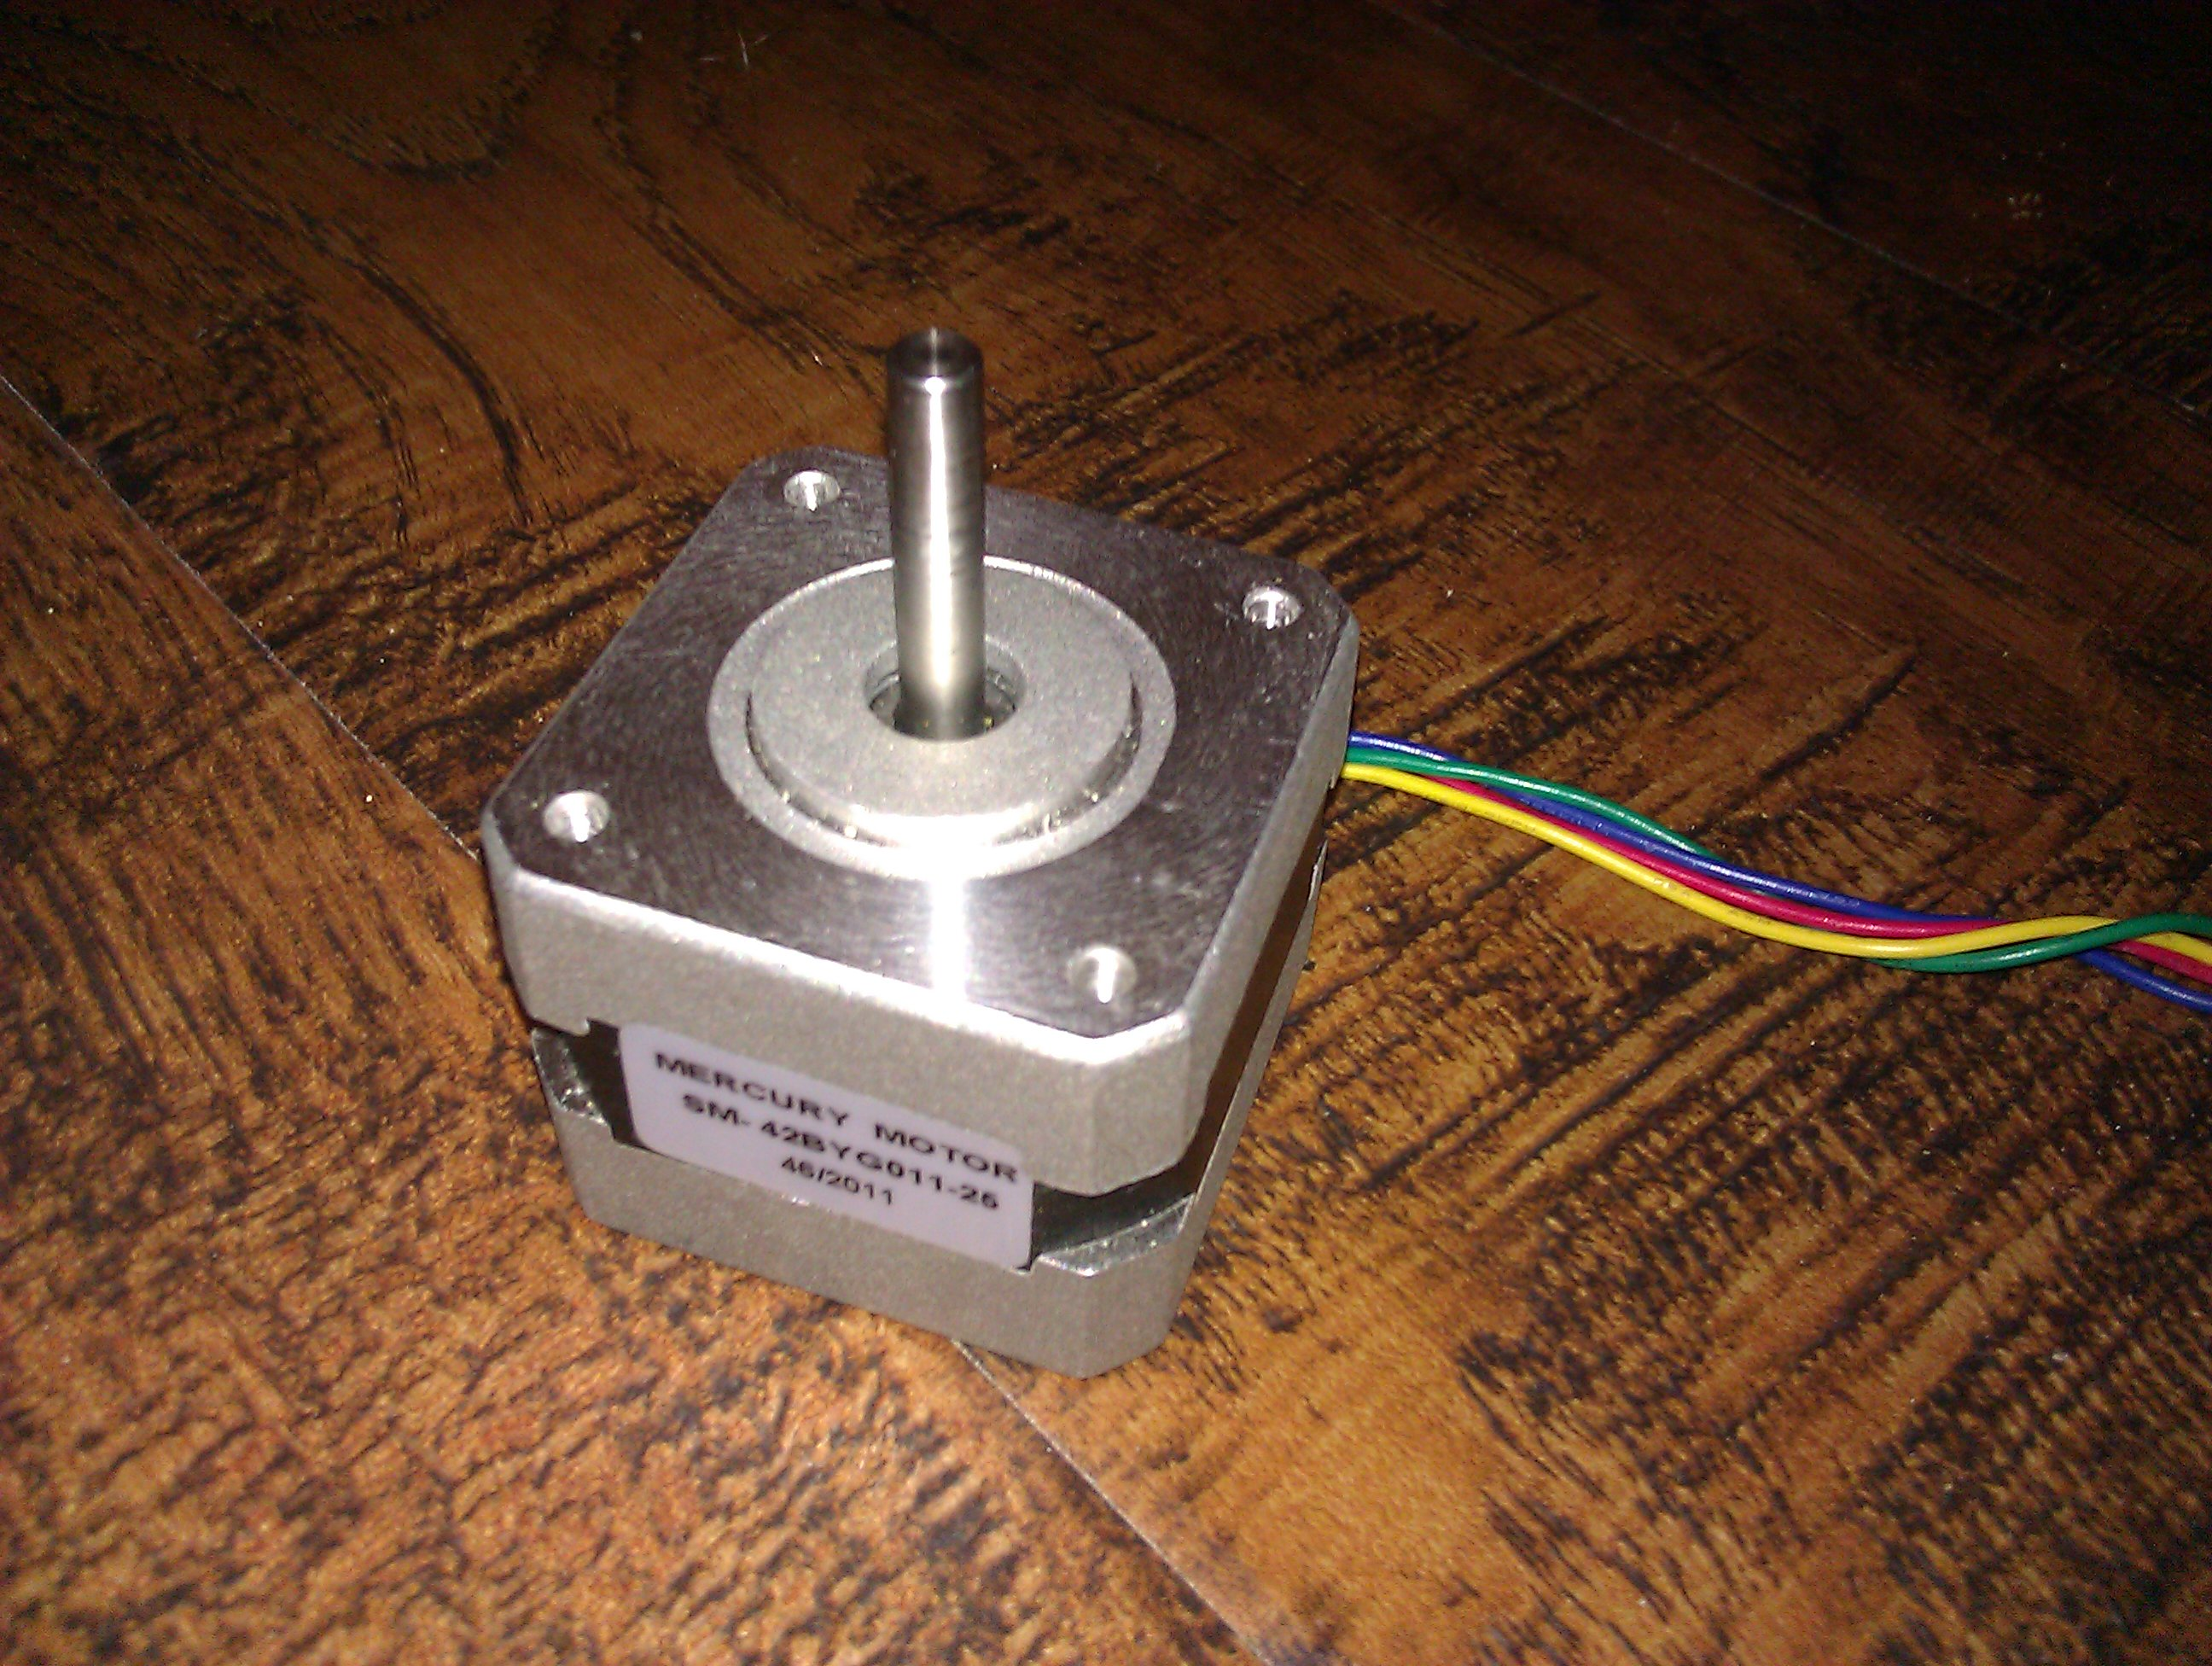
\includegraphics[width=3.0in]  {Images/small-stepper.jpg}
        \caption{Chosen Stepper Motor}
        \label{Chosen Stepper Motor}
\end{figure}
\begin{figure}[h]
\centering
        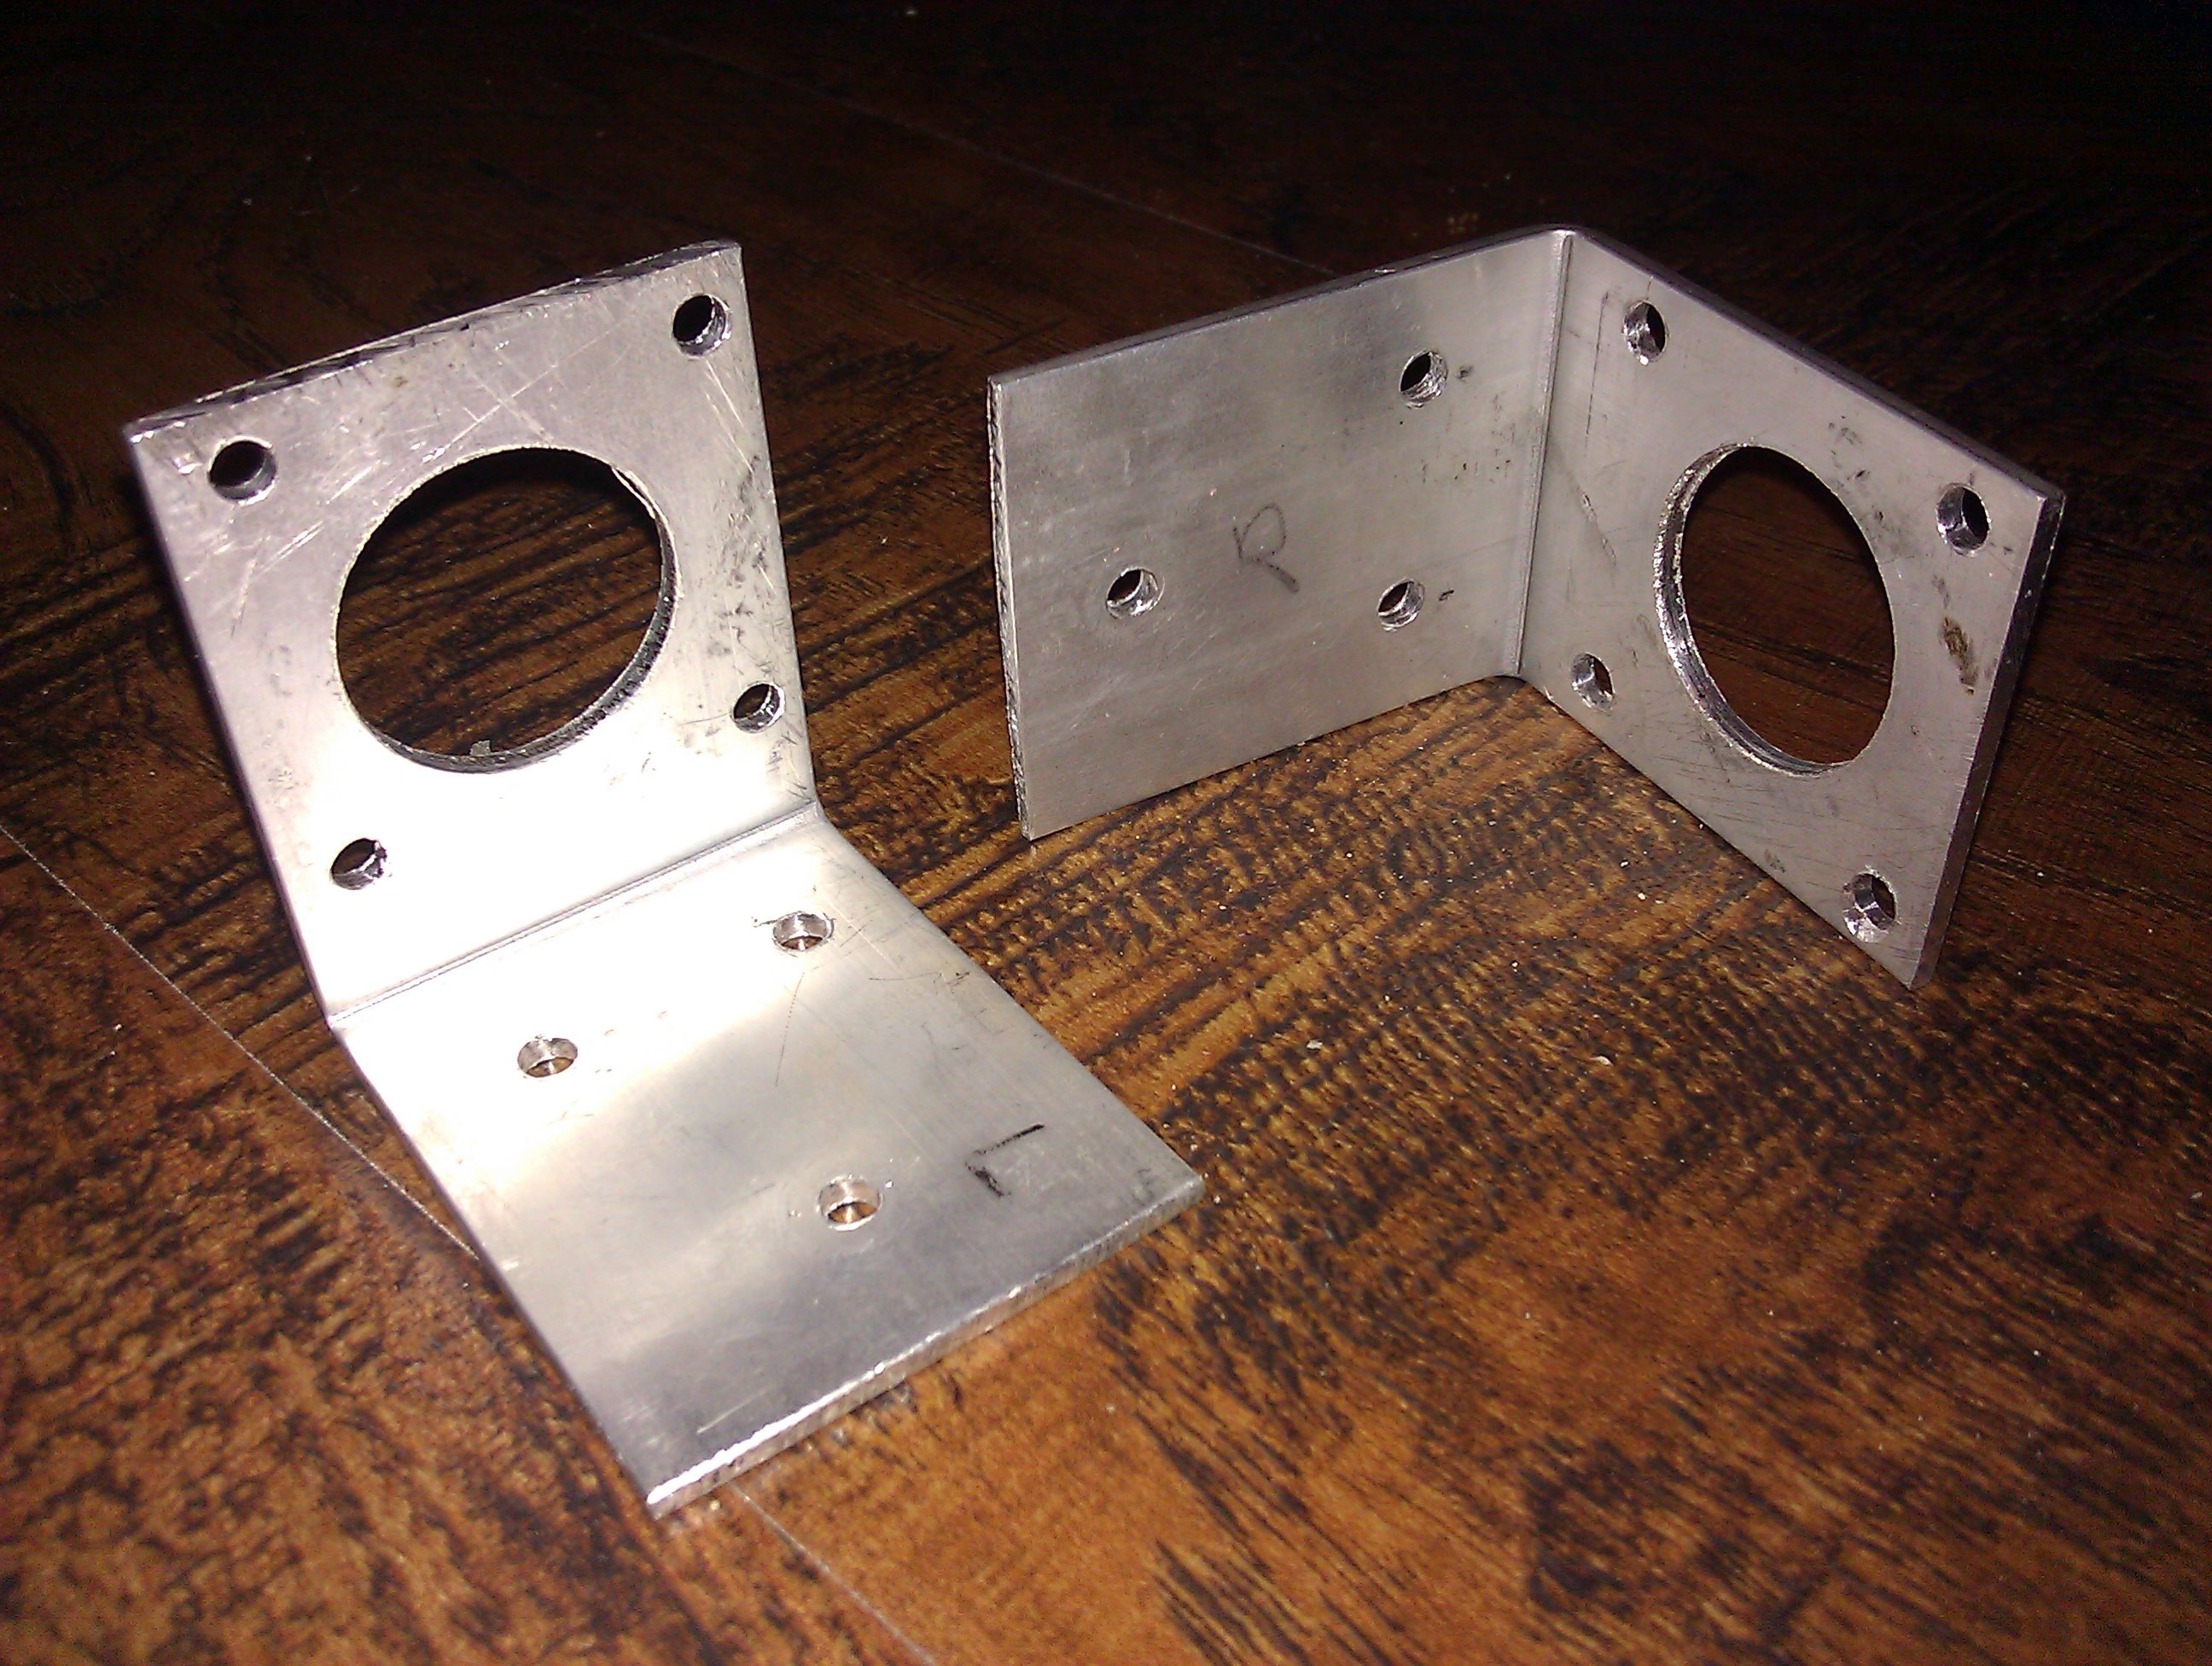
\includegraphics[width=3.0in]  {Images/motor-mount-1.jpg}
        \caption{Motor Mounts}
        \label{Motor Mounts}
\end{figure}
\\These mounts are just the cut strips of aluminium that have been bent so that they form a 90 degree angle and holes drilled through them to accomodate the motor drive shaft and for screw holes to attach these mounts to the baseplate.
\\Another alteration to the original design is the fact that I have chosen to use only two drive wheels instead of the four shown in the design document.  The reasoning for this was that it is easier to turn with just the two wheels as it will be able to almost turn on the spot rather than having to perform a multi directional turn, moving backwards and forwards turning a different direction for each just like how a driver would turn a car around in a tight space.
\\Now that the design has been reduced from four drive motors down to only two it will need some other wheels to keep the robot stable.  A single rear caster wheel worked well for the prototype and if I went with two rear stabalising wheels then the car turning in a tight space issue would still apply and because of this a single wheel has been chosen.
\\This wheel again has been mounted on a strip of aluminium bolted hanging over the rear end of the also aluminium baseplate.
\begin{figure}[h]
\centering
        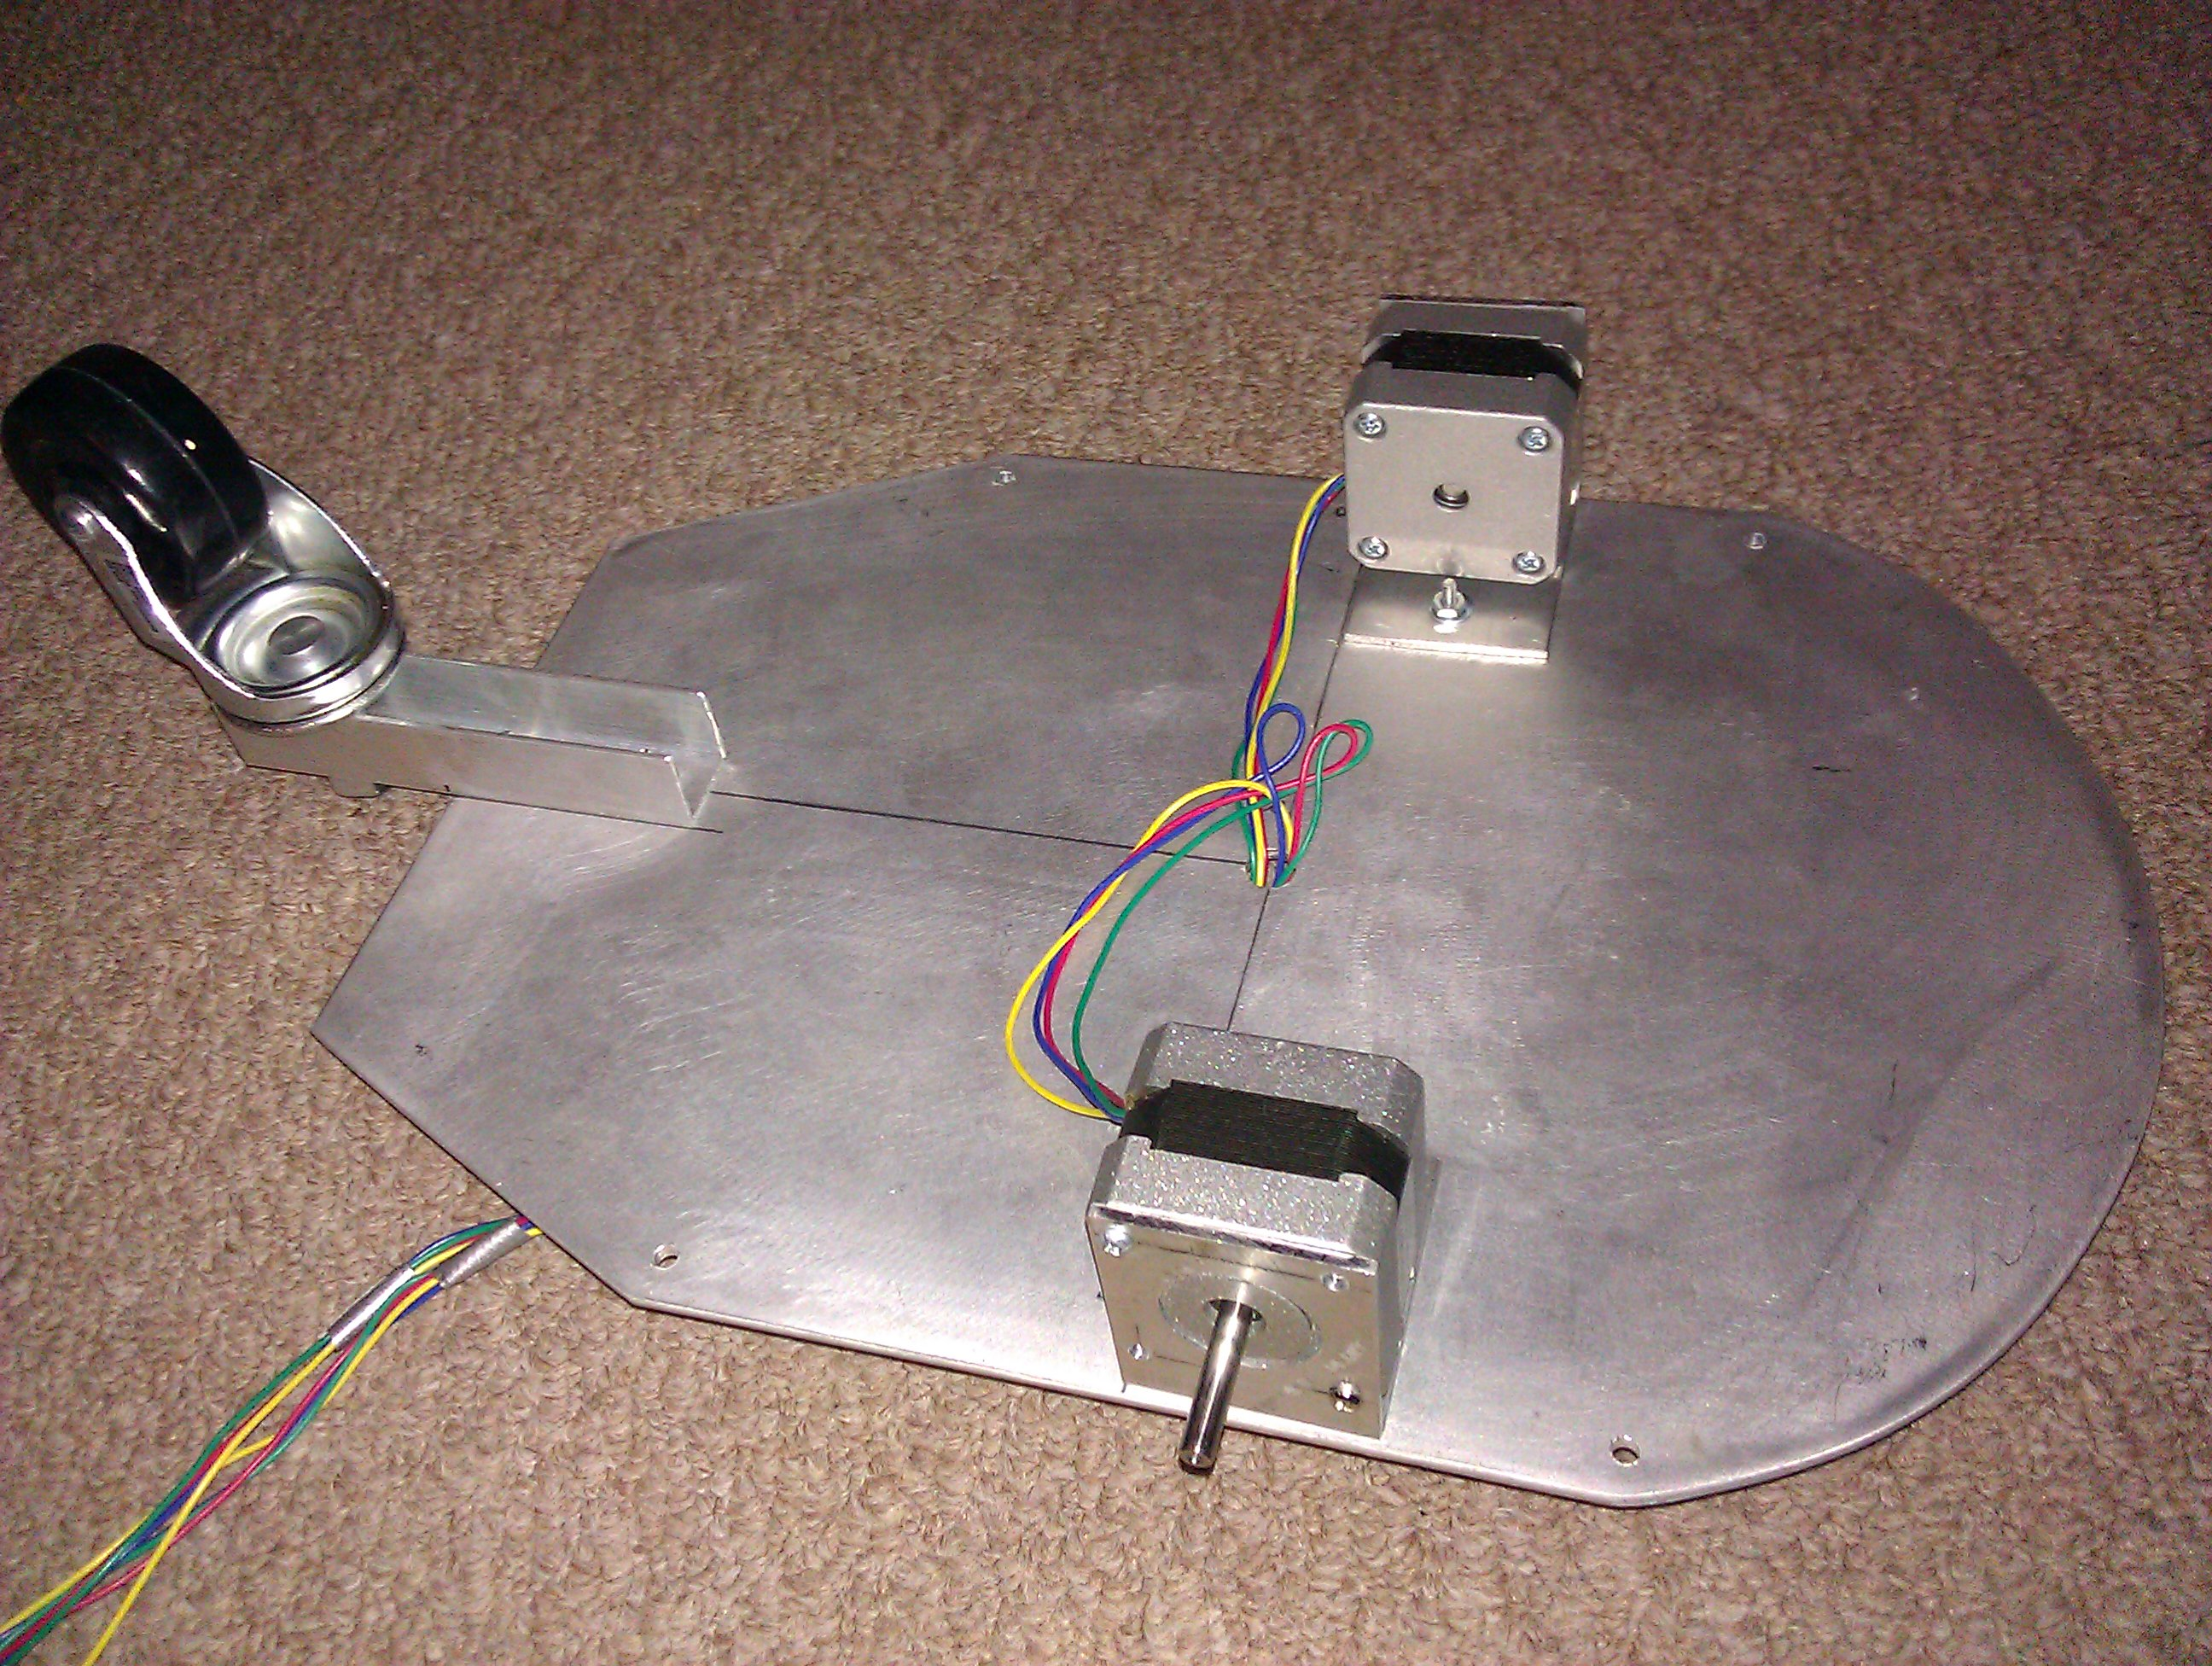
\includegraphics[width=3.0in]  {Images/baseplate-underside.jpg}
        \caption{Baseplate Underside}
        \label{Baseplate Underside}
\end{figure}
Having chosen to use stepper motors for the reason of increased accuracy over the less precise DC motors it would be a bad idea to go for wheels which have insufficient traction and as such I chose offroad style wheels which have a wide and deep tread with spikes for additional grip.
\\These wheels measure 120mm in diameter and 60mm wide which results in it being harder to turn and will require a stronger motor to move.
\begin{figure}[h]
\centering
        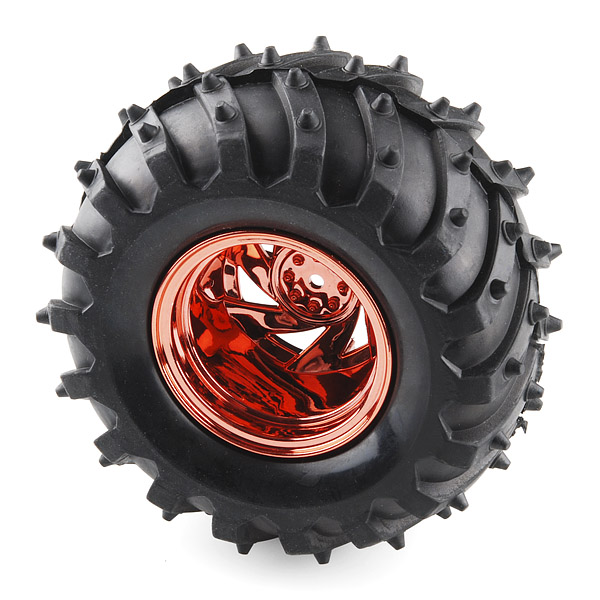
\includegraphics[width=3.0in]  {Images/wheel-offroad.jpg}
        \caption{Offroad Wheel - sparkfun.com}
        \label{Offroad Wheel}
\end{figure}
\subsection{Manufacturing Parts}
Before starting this project I spent some time building a three dimensional printer.  This device is just like an ordinary printer but creates the dimentional physical objects.
\\An ordinary printer uses a print head to dispense ink onto a sheet or paper or card to leave a permanant mark on it which after a lot of small apllications of the ink will build up letters or a picture.  A three dimensional printer works in a very similar way.  Plastic is fed into the print head where it is heated up above the melting point of whichever plastic is being used then extruded out onto a heated print bed.  While this melted plastic is being extruded the head is being moved around to draw out the shape of whatever is being printed.  This is currently still essentially two dimensional, what happens next is that once the first layer is ifnished with either the print head moves up or the print bed moves down and the next layer is started.  This is how this type of printer works, after the first layer is printed onto the heated bed, the next layer is printed on top of the previous one.  This process continues as many times as neccesary until the layers are built up into the full object.
\\This process is very usefull as it wastes no materials as it is an additive proccess as opposed to other computer aided manufacturing methods which are generaly subtractive.  This means that other machines cut away excess off of a block of a selected material when this printer only adds material that is needed.
\\The reason I built this printer is to produce one off custom components for any project I might need such a capability.  Instead of trying to source the exact component I want of the right size and shape, or having to modify something else, the idea of just being able to create a three dimensional model on a computer of the object I want to create and then just be able to make it at a whim is a very attractive prospect.  These parts do not only have to be plastic, there are 3D printers can can even print metal, some of these parts are used in aircraft and even formula one cars.  The printer I built had many printed components as parts of its own construction.  These parts were made out of a blue plastic.
\begin{figure}[h]
\centering
        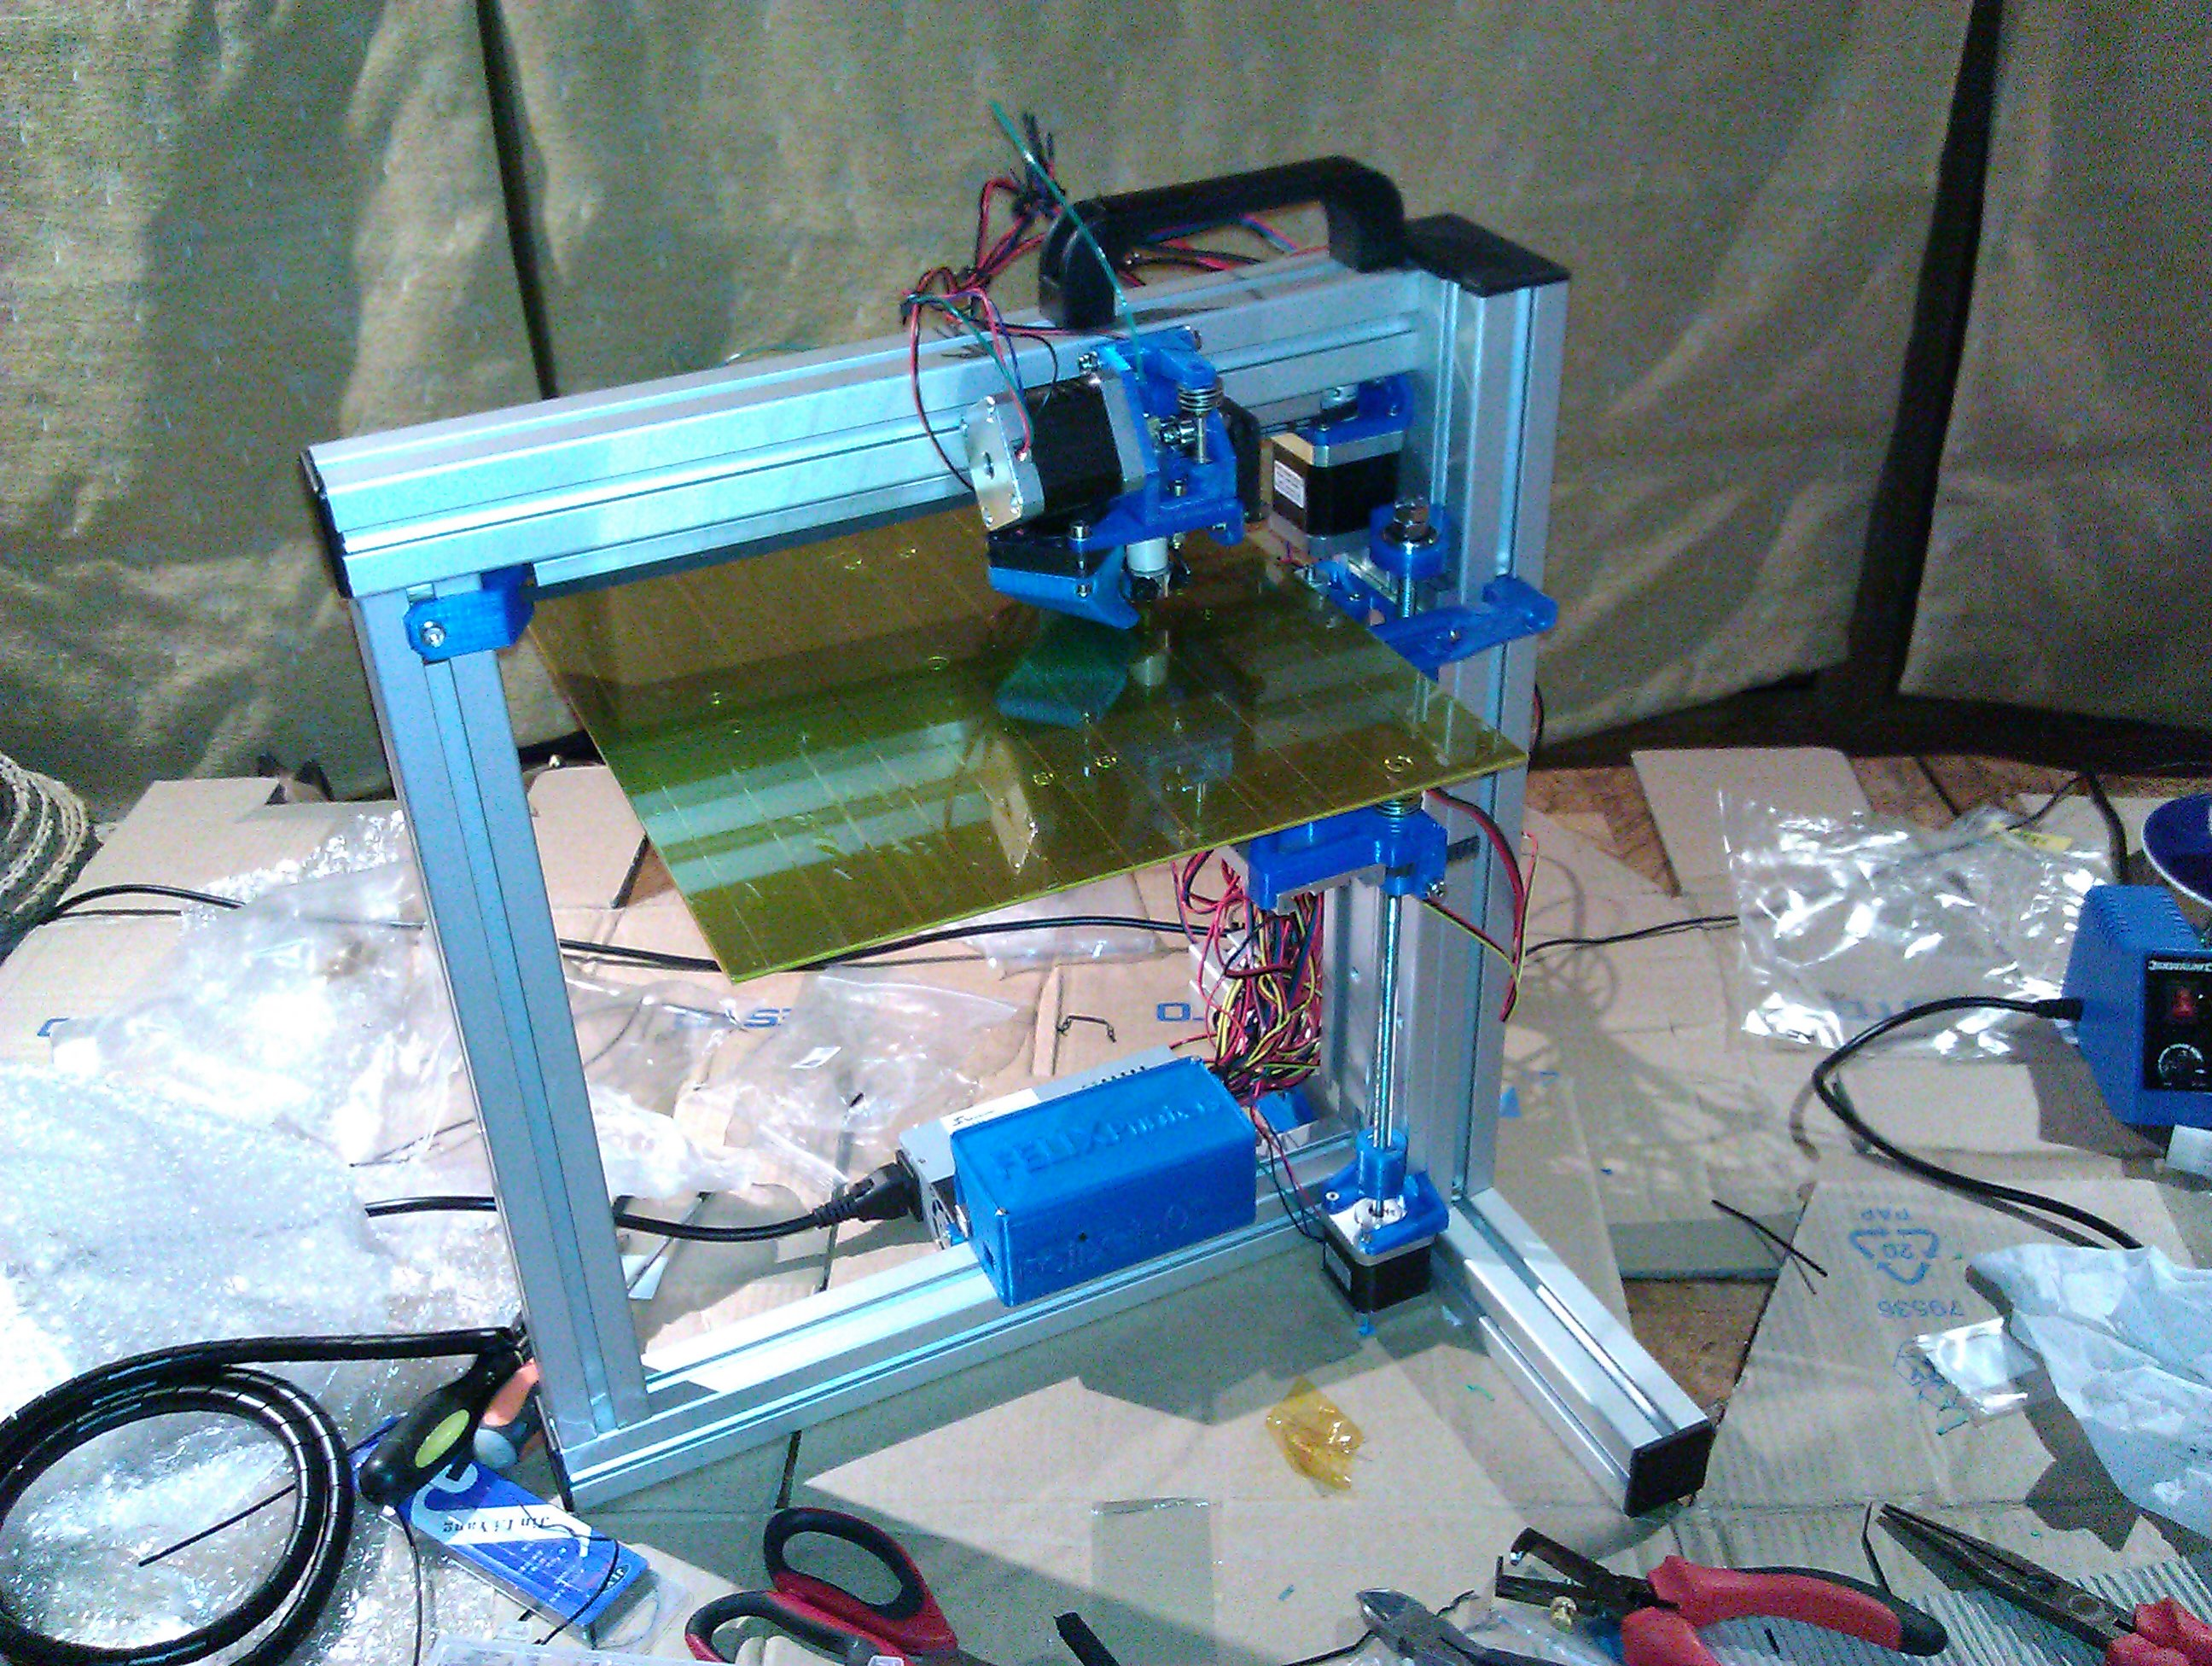
\includegraphics[width=5.0in]  {Images/printer.jpg}
        \caption{3D Printer}
        \label{3D Printer}
\end{figure}
\\The first component for the robot that I constructed with this printer is a mount for the microcontroller.  The mount is use to attach the component to the chassis and to insulate it from the metal base to avoid short circuits between varies part of the component and between it and other components that may also be mounted on the same base plate.  This mounting plate was constructed by the printer in less than half an hour and weighing under 25 grams and costing me less than 50 pence.
\begin{figure}[h]
\centering
        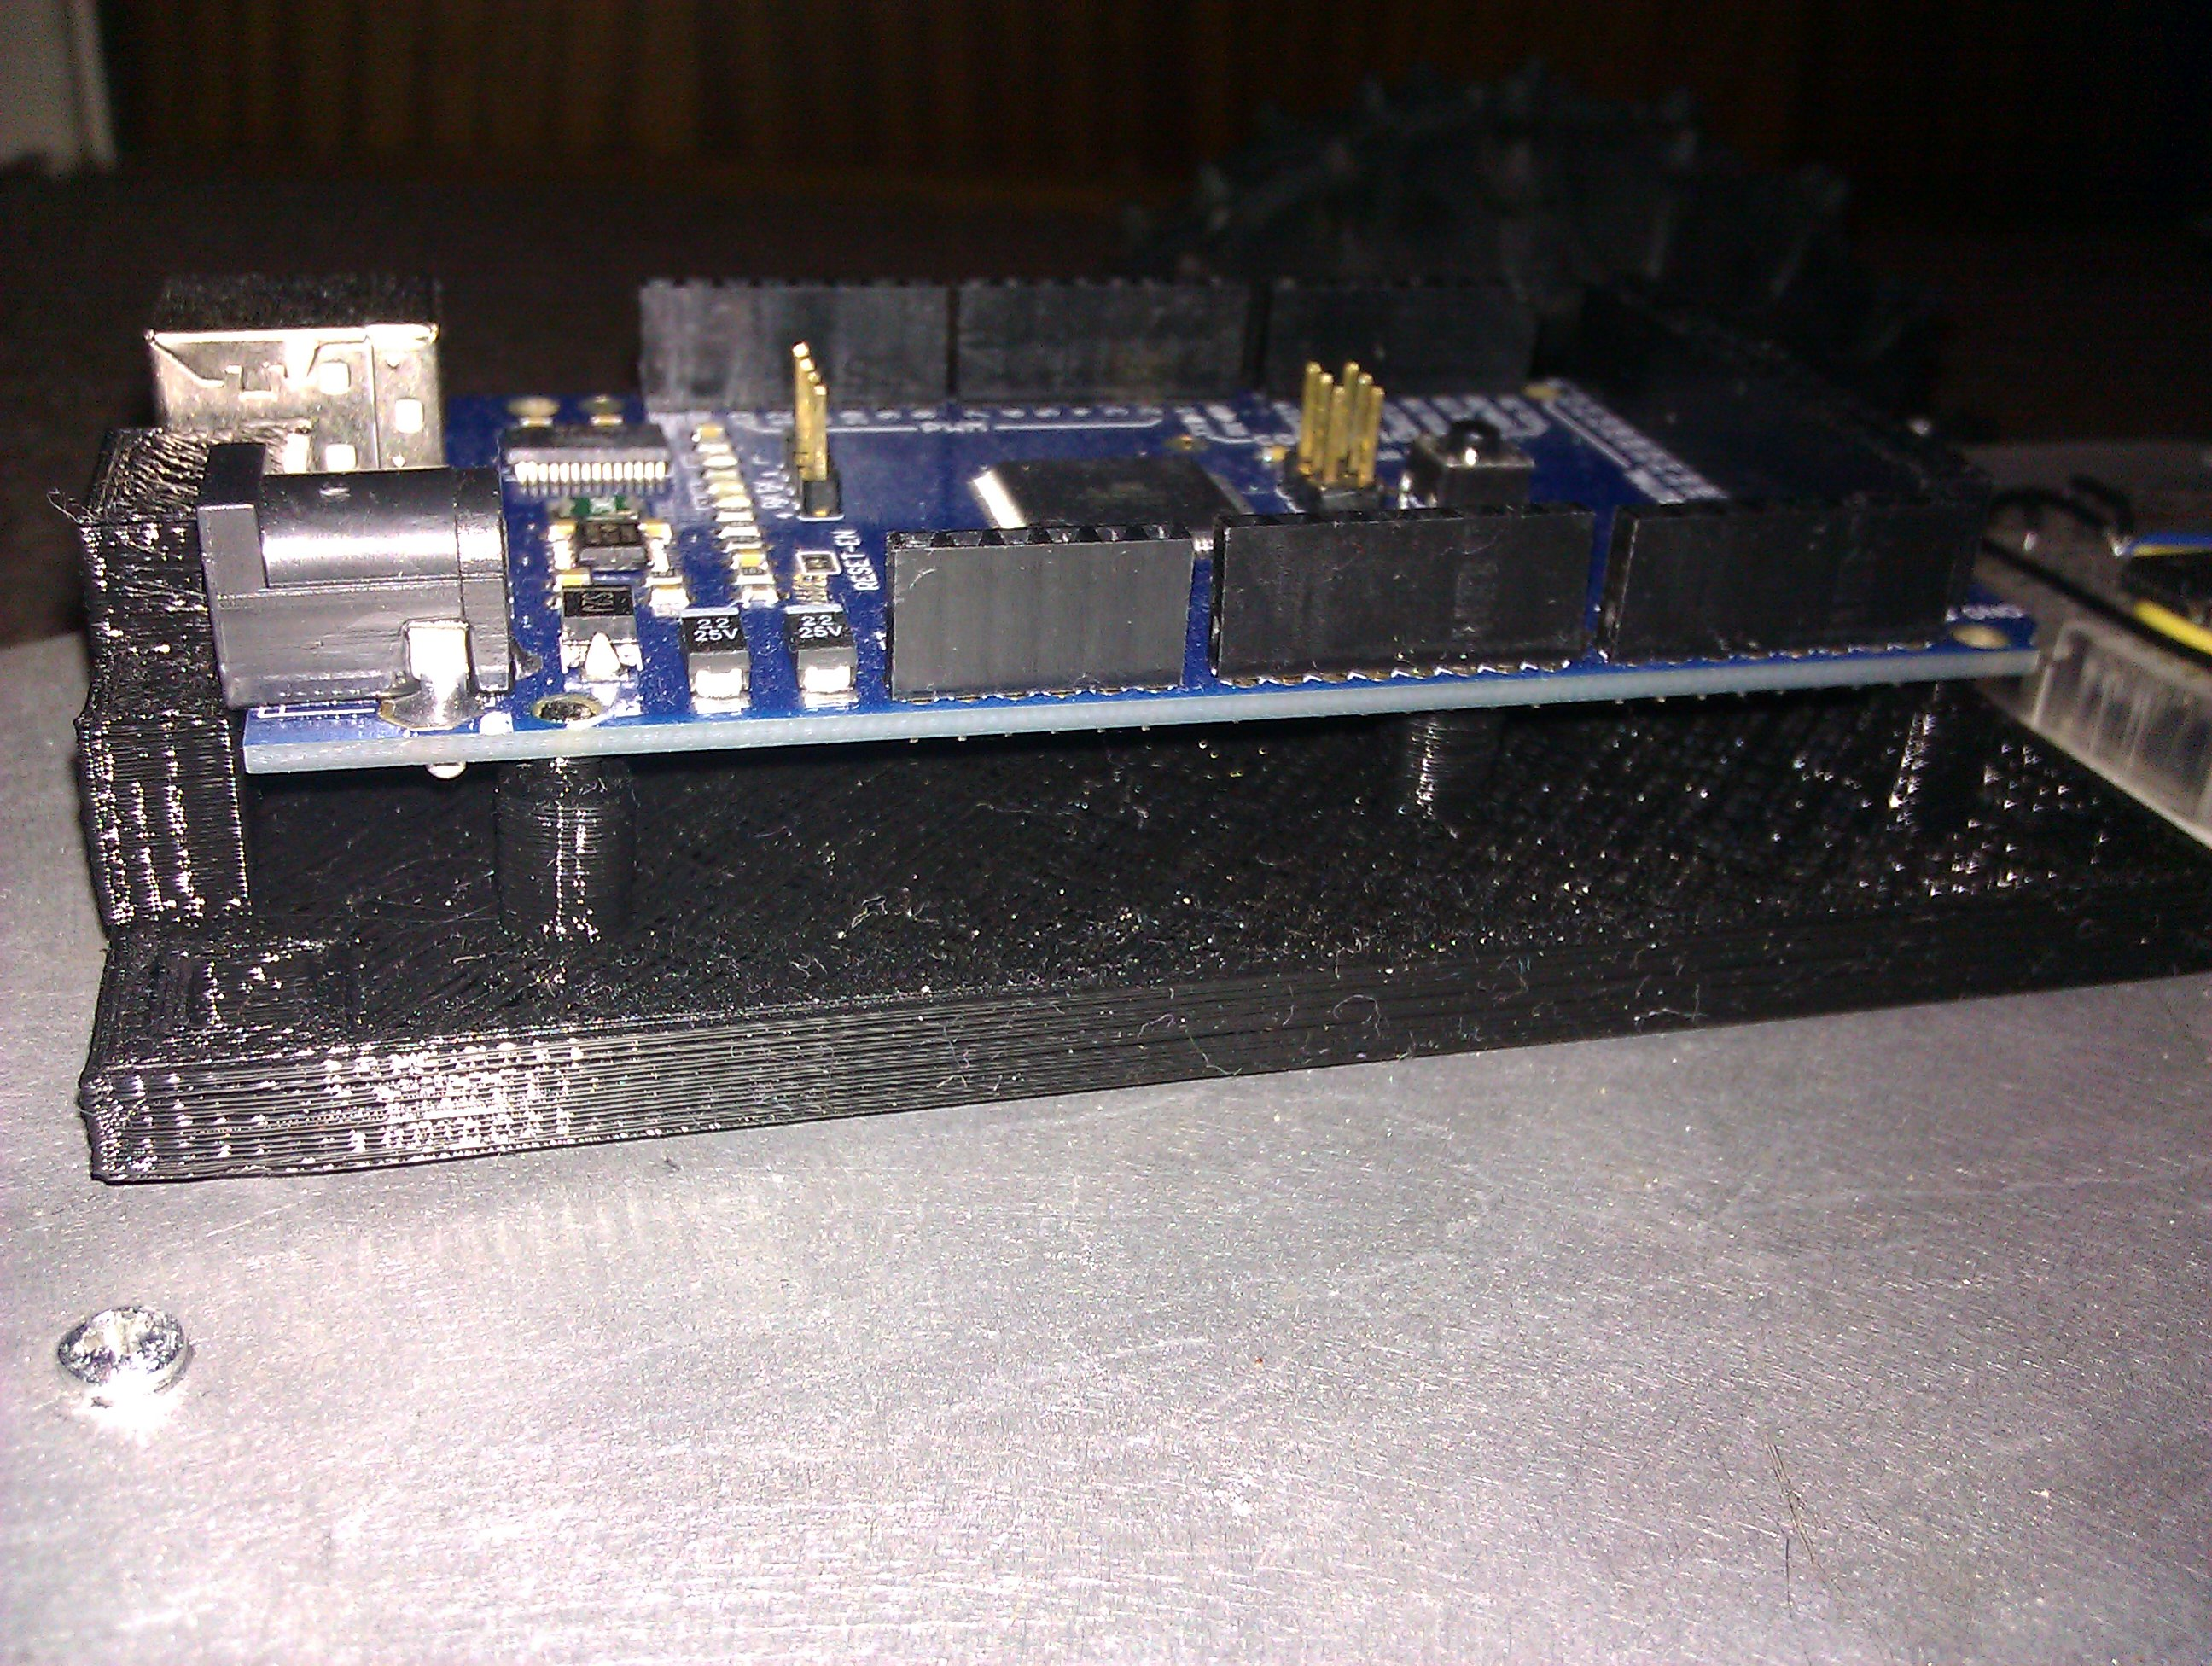
\includegraphics[width=5.0in]  {Images/printed-mount.jpg}
        \caption{Printed Mounting Plate}
        \label{Printed Mounting Plate}
\end{figure}

\chapter{Testing}

%Detailed descriptions of every test case are definitely not what is required here. What is important is to show that you adopted a sensible strategy that was, in principle, capable of testing the system adequately even if you did not have the time to test the system fully.

%Have you tested your system on 'real users'? For example, if your system is supposed to solve a problem for a business, then it would be appropriate to present your approach to involve the users in the testing process and to record the results that you obtained. Depending on the level of detail, it is likely that you would put any detailed results in an appendix.

\section{Overall Approach to Testing}
Testing any complex hardware of software system is a critical process because if there are any major points of failure the whole system could cease to operate.  Time does not always permit this but at least some general testing of all systems should be carried out to highlight any obvious problems.
\section{Automated Testing}
Automated testing is a very good process to be using as the system being developed is tested and the results of these tests whether they be positive or if they highlight problems with the system all without the developer having to do anything after the initial setup of this testing process.
\\Due to the embedded nature of this project, automated testing is very limited.  As there is no simulator for an arduino microcontroller and all the various components that can be used in conjunction with one, no automated testing of this can be achieved without a far more complex hardware system which somehow can test other hardware configurations.  The only part of the system that can be automatically tested with any degree of reliability is to parse the software code and check is it is syntactically valid.
\subsection{System Tests}
These are written to test each individual part of the project.  This starts with testing if the code validates.  A compiler is used to validate this and a compiler is another program that checks if code will actually work, not necessarily for its intended purpose but just check that it does not have a major flaw that will stop the finished program from running at all and converts it into either a binary capable of being run as an executable program or into another language.  This compiled code is what will run on the hardware itself rather than through an interpreter which is another program that interprets what the code is trying to do and runs that.
\\The next stage of testing is to check that the software for each individual hardware interaction works as expected.  This includes checking that when the code tells a motor to turn in a specific direction that it actually turns as it is told to.  A motor is laid out on a workbench, hooked up to the microcontroller and told to turn.  If it does as expected then the test will be considered as passed, otherwise it will be considered as failed and debugging will be required before running the tests again.
\\Similar tests will be run on the sensors with then placed at set distance intervals from objects and tested to see if the recorded distance measured by the sensor is the same as the real world measurement specifies.
\begin{figure}[h]
\centering
        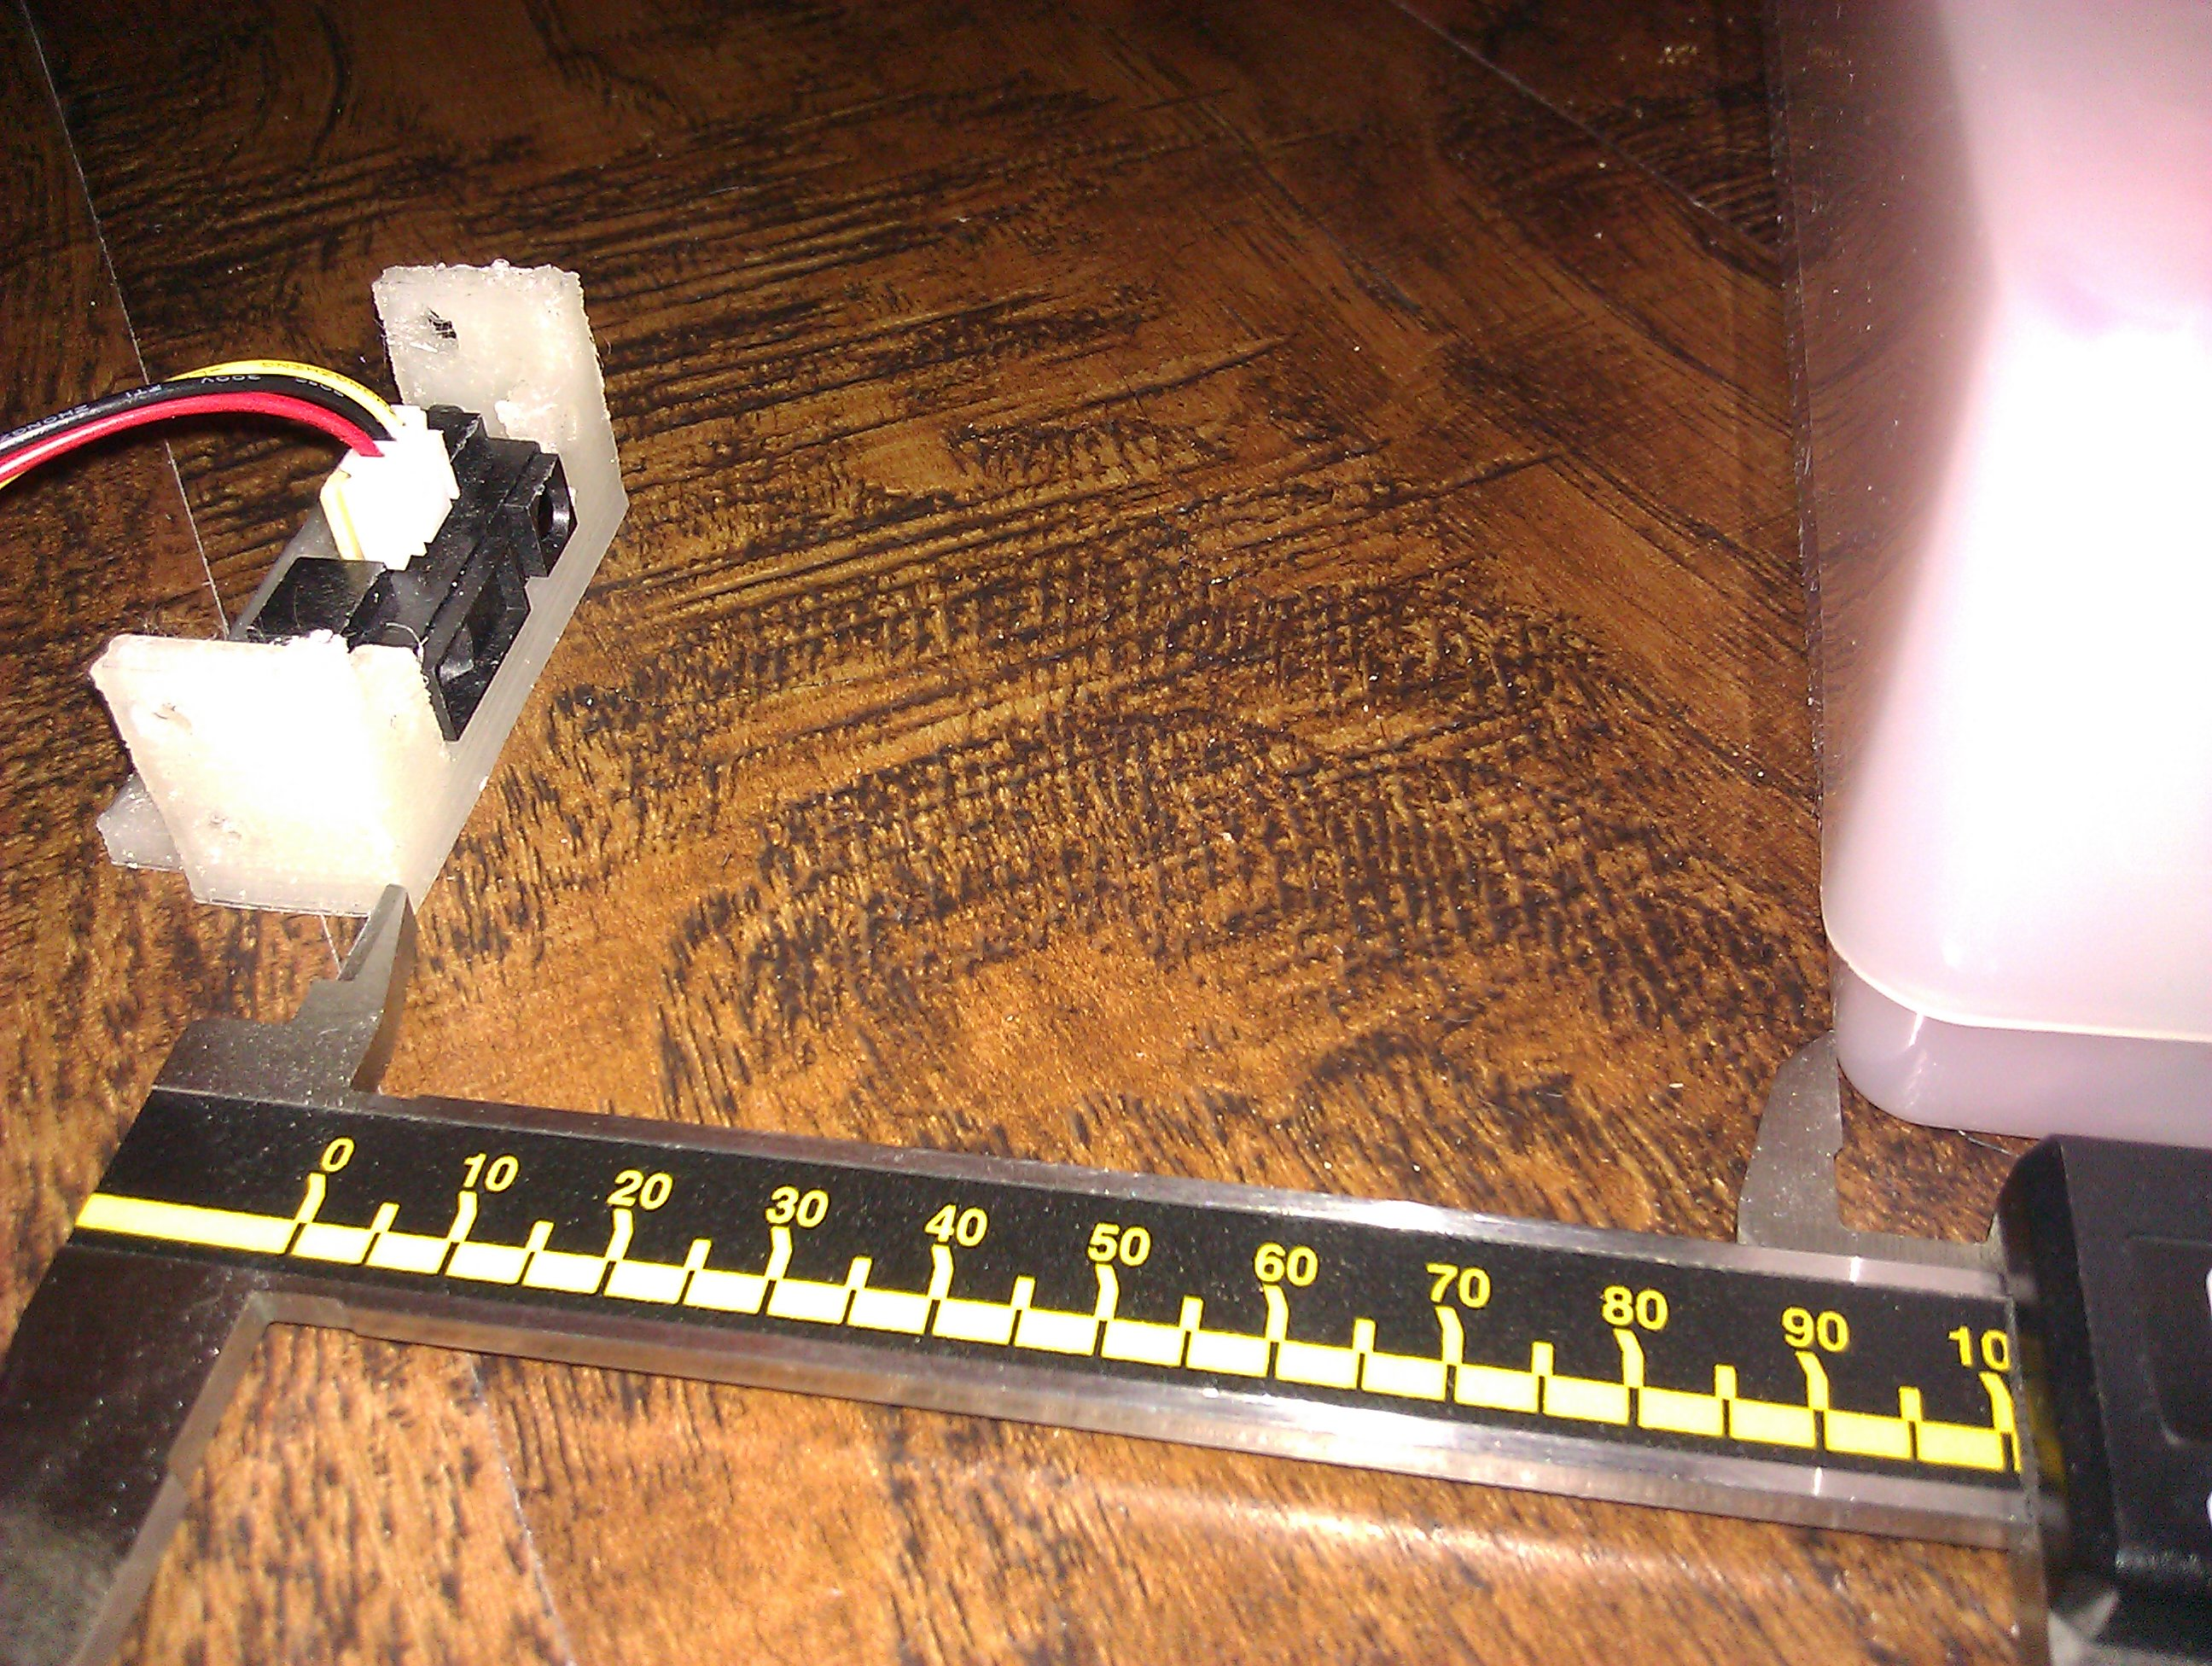
\includegraphics[width=4.0in] {Images/ir-measure-2.jpg}
        \caption{Infrared Distance Test}
        \label{Infrared Distance Test}
\end{figure}
\subsection{User Interface Testing}
The only user interface on the robot is a button to apply or cut off power to the system and an activity readout over a serial communication line.  This communication can either be over a USB (universal serial bus) cable or over some form of wireless serial such as bluetooth or the xbee module I am using.
\subsection{Stress Testing}

\section{Integration Testing}


\chapter{Evaluation}

%Examiners expect to find in your dissertation a section addressing such questions as:

%\begin{itemize}
%   \item Were the requirements correctly identified?
%   \item Were the design decisions correct?
%   \item Could a more suitable set of tools have been chosen?
%   \item How well did the software meet the needs of those who were expecting to use it?
%   \item How well were any other project aims achieved?
%   \item If you were starting again, what would you do differently?
%\end{itemize}

%Such material is regarded as an important part of the dissertation; it should demonstrate that you are capable not only of carrying out a piece of work but also of thinking critically about how you did it and how you might have done it better. This is seen as an important part of an honours degree.
%There will be good things and room for improvement with any project. As you write this section, identify and discuss the parts of the work that went well and also consider ways in which the work could be improved.
%The critical evaluation can sometimes be the weakest aspect of most project dissertations. We will discuss this in a future lecture and there are some additional points raised on the project website.

The final product met what was outlined in the abstract.  This being that a robot was built that could move around an environment under it's own power, detect and avoid approaching obstacles.
\\\\It does not perform this task as reliably as it was expected to from the initial description, the main issue being with the drive system.  I had under estimated how much torque the motors would require to move the total weight of the finished robot, this was not identified correctly in the initial design.  This issue was addressed later on in the project implementation but was not fully corrected, the robot does move but it only takes a moderate incline like a ramp to make the robot struggle to move again.  Choosing stepper motors alone was a bad design decision and in hindsight I should have used a gear system to gain the extra torque that it needed to handle movement up an incline.
\\\\The sensor pair worked well to validate each other in the event of interference or an unfavourable environment.  With the robot only being able to see in two very narrow straight lines out in front of it, I would have liked to add more sensor pairs to get a wider view of the environment.  A wider view would allow for better calculating which direction had the least obstacles in and to move accordingly.
\\Extra sensor pairs would be arranged in a circle around the robot to form a halo.  This would still only give narrow points of view of the environment.  I could possibly mount a sensor pair on a servo controller pan and tilt mount, this could then point the sensors at any angle from the robot and take readings.  This would work but it would also be very slow and impractical.  A camera would also be a good solution I would consider for generating a more accurate map of the robot's surrounding environment to better work out where to go.  The camera solution will require far more processing than the current sensor solution but has a much higher resolution.
\\\\I think that the tools I used to complete this project were appropriate, these being the Arduino development environment, version control system used to develop the software and the various hardware tools used to create the physical robot.  A different version control system could have been used to maintain the code such as subversion or mercurial but this project did not actually require any complex features of these systems apart from merging.  All of the merges that took place were simple and very easy to do, but that may have been due to how good Git is at performing this function.
\\As stated previously the project aims were met but not to as high of a standard as I had hoped for.  The robot has to stop moving to take sensor readings as the microcontroller is not capable of multitasking, this is an issue as it puts more strain on the motors with this stop and start behaviour.
\\\\If I were to start this project again from scratch I would seperate the main tasks such as motor control, sensor readings and decision making each to their own processor.  By this I mean that each subsystem would have it's own microcontroller and a central unit would tell them what to do.  This would mean that the control unit can tell the robot to move forwards unti told otherwise and the sensor subsystem could take all the readings it wants without disrupting the movements of the robot.  I would also use a sensor system with higher resolution of the environment and which is more reliable such as a camera or a pair of cameras to be able to detect depth.  A laser scanner would also be a good sensor to have but they are very expensive and require even more processing than the camera.
\\The robot is very heavy due to the amount of aluminium used in the construction of the chassis and the mounts, this could be greatly reduced by using the 3D printer to fabricate a chassis.  This chassis would be different from one made out of cut sheets of plastic because it can be made hollow with an internal structure such as a honeycomb weave to keep the strength near to that of a solid sheet.  This method would reduce the cost and be made to whichever specifications are required.
\\\\Overall the project met it's basic aim but has much room for improvment and expansion by building upon all of the mentioned system alterations.
% add any additional chapters here

\setemptyheader
\addcontentsline{toc}{chapter}{Appendices}
\chapter*{Appendices}
\pagebreak

% start the appendix - sets up different numbering
\fancypagestyle{plain}{%
%\fancyhf{} % clear all header and footer fields
\fancyhead[L]{\textsl{Appendix\ \thechapter}}
\fancyhead[R]{\textsl{\leftmark}}}

\appendix
\fancyhead[L]{\textsl{Appendix\ \thechapter}}
\fancyhead[R]{\textsl{\leftmark}}
\fancyhead[C]{}
\fancyfoot[C]{\thepage}
\renewcommand{\headrulewidth}{0.4pt}
\renewcommand{\chaptermark}[1]{\markboth{#1}{}}

\fancyhead[L]{\textsl{Appendix\ \thechapter}}
\fancyhead[R]{\textsl{\leftmark}}
\fancyfoot[C]{{\thepage} of \pageref{LastPage}}

% include any appendices here
\chapter{Third-Party Code and Libraries}

%If you have made use of any third party code or software libraries, i.e. any code that you have not designed and written yourself, then you must include this appendix. 

As has been said in lectures, it is acceptable and likely that you will make use of third-party code and software libraries. The key requirement is that we understand what is your original work and what work is based on that of other people. 

Therefore, you need to clearly state what you have used and where the original material can be found. Also, if you have made any changes to the original versions, you must explain what you have changed.
The main piece of thrid party software that I used is the Arduino integrated development environment.  This is a software package used to write programs, compile them and deploy them onto the arduino microcontroller series.
\\This software includes a collection of libraries to be used withe the arduino hardware to aid in the development of programs for it.  The only one of these libraries I use is for serial communication fo the sensor data base to a human readable terminal.

\chapter{Code samples}

\section{Random Number Generator}

The Bayes Durham Shuffle ensures that the psuedo random numbers used in the simulation are further shuffled, ensuring minimal correlation between subsequent random outputs \cite{NumericalRecipes}.

\begin{verbatim}
 #define IM1 2147483563
 #define IM2 2147483399
 #define AM (1.0/IM1)
 #define IMM1 (IM1-1)
 #define IA1 40014
 #define IA2 40692 
 #define IQ1 53668
 #define IQ2 52774
 #define IR1 12211
 #define IR2 3791
 #define NTAB 32
 #define NDIV (1+IMM1/NTAB)
 #define EPS 1.2e-7
 #define RNMX (1.0 - EPS)
 
 double ran2(long *idum)
 {
   /*---------------------------------------------------*/
   /* Minimum Standard Random Number Generator          */
   /* Taken from Numerical recipies in C                */
   /* Based on Park and Miller with Bays Durham Shuffle */
   /* Coupled Schrage methods for extra periodicity     */
   /* Always call with negative number to initialise    */
   /*---------------------------------------------------*/	
 
   int j;
   long k;
   static long idum2=123456789;
   static long iy=0;
   static long iv[NTAB];
   double temp;
 
   if (*idum <=0)
   {
     if (-(*idum) < 1)
     {
       *idum = 1;
     }else
     {
       *idum = -(*idum);
     }
     idum2=(*idum);
     for (j=NTAB+7;j>=0;j--)
     {
       k = (*idum)/IQ1;
       *idum = IA1 *(*idum-k*IQ1) - IR1*k;
       if (*idum < 0)
       {
         *idum += IM1;
       }
       if (j < NTAB)
       {
         iv[j] = *idum;
       }
     }
     iy = iv[0];	
   }
   k = (*idum)/IQ1;
   *idum = IA1*(*idum-k*IQ1) - IR1*k;
   if (*idum < 0)
   {
     *idum += IM1;
   }
   k = (idum2)/IQ2;
   idum2 = IA2*(idum2-k*IQ2) - IR2*k;
   if (idum2 < 0)
   {
     idum2 += IM2;
   }
   j = iy/NDIV;
   iy=iv[j] - idum2;
   iv[j] = *idum;
   if (iy < 1)
   {
     iy += IMM1;
   }
   if ((temp=AM*iy) > RNMX)
   {
     return RNMX;
   }else
   {
     return temp;	
   }
 }
 
\end{verbatim}



\fancypagestyle{plain}{%
   \fancyhead{} %[C]{Annotated Bibliography}
   \fancyfoot[C]{{\thepage} of \pageref{LastPage}} % except the center
   \renewcommand{\headrulewidth}{0pt}
   \renewcommand{\footrulewidth}{0pt}
}

\setemptyheader

\nocite{*} % include everything from the bibliography, irrespective of whether it has been referenced.

% the following line is included so that the bibliography is also shown in the table of contents. There is the possibility that this is added to the previous page for the bibliography. To address this, a newline is added so that it appears on the first page for the bibliography.
\addcontentsline{toc}{chapter}{Annotated Bibliography} % Adds References to contents page

%
% example of including an annotated bibliography. The current style is an author date one. If you want to change, comment out the line and uncomment the subsequent line. You should also modify the packages included at the top (see the notes earlier in the file) and then trash your aux files and re-run.
\bibliographystyle{authordate2annot}
%\bibliographystyle{IEEEannot}
\renewcommand{\bibname}{Annotated Bibliography}
\bibliography{References/references} % References file


\end{document}
